% #####################################################################
% #####################################################################
% ##                                                                 ##
% ##                                                                 ##
% #####################################################################
% #####################################################################
% #####################################################################
\documentclass[a4paper,landscape,6pt]{article}
\usepackage[utf8]{inputenc}
\usepackage[ngerman]{babel}
\usepackage[top=2.0cm,bottom=1.5cm,left=1.0cm,right=1.0cm]{geometry}
\usepackage{enumitem}
\usepackage{graphicx}
\usepackage{amsfonts}
\usepackage{amsmath}
\usepackage{sectsty}
\usepackage{colortbl}
\usepackage{cancel}
\usepackage{listings}
\usepackage{color}
\usepackage{epstopdf}
\usepackage{fancyhdr}
\usepackage{tikz}
\usepackage{multicol}


\RequirePackage{mTex/mTex_boxes}
\RequirePackage{mTex/colors}
%\geometry{a4paper,landscape, left=5mm,right=5mm, top=20mm, bottom=5mm, asymmetric}

\newcommand{\ma}[1]{\ensuremath{\boldsymbol {#1}}}								% Matrixsymbol
\newcommand{\mat}[1]{\ensuremath{\begin{bmatrix} #1 \end{bmatrix}}}				% Matrix
\newcommand{\tma}[3]{\ensuremath{{}_{#1} \ma #2_#3 }}							% Trafomatrix
\renewcommand{\vec}[1]{\ensuremath{\boldsymbol {#1}}}							% Vektor fett und unterstrichen
\newcommand{\vect}[1]{\ensuremath{\begin{pmatrix} #1 \end{pmatrix}}}			% Vector mit runden Klammern
\newcommand{\mvect}[1]{\ensuremath{\left.\begin{matrix} #1 \end{matrix}\right]}}% Matrixvector
\newcommand{\diff}[2]{\frac{\mathrm{d}#1}{\mathrm{d}#2}}
\newcommand{\partdiff}[2]{\frac{\partial #1}{\partial #2}}						% partielle Ableitung
\renewcommand{\exp}[1]{\textrm{e}^{#1}}											% e-Funktion
%\newcommand\tab[1][1cm]{\hspace*{#1}}
\newcommand{\ul}[1]{\underline{#1}}


\setlist{itemsep=.01mm}
\setenumerate{label=\emph{\arabic*})}
\setlength{\columnsep}{1cm}
\parindent 0mm

\partfont{\huge}
\sectionfont{\Large \sc\bf}
\subsectionfont{\normalsize}
\subsubsectionfont{\small\textit}

\pagestyle{fancy}
\lhead[\leftmark]{Systeme der Signalverarbeitung}
\chead[\leftmark]{Stand: \today}
\rhead[\leftmark]{Johannes Teutsch}
\lfoot[\leftmark]{}
\cfoot[\leftmark]{Keine Garantie auf Vollständigkeit und Richtigkeit!}
\rfoot[\leftmark]{\thepage}
\renewcommand{\headrulewidth}{0.5pt}
\renewcommand{\footrulewidth}{0.5pt}

%\newcommand*\kreis[1]{\unitlength1ex\begin{picture}(2.5,2.5)%
%\put(0.75,0.75){\circle{3}}\put(0.7,0.7){\makebox(0,0){#1}}\end{picture}}

\DeclareMathOperator{\cov}{cov}
\DeclareMathOperator{\str}{str}
\DeclareMathOperator{\val}{val}

\newenvironment{abc}{\begin{enumerate}[label={\alph*)}]}{\end{enumerate}}
\newenvironment{iii}{\begin{enumerate}[label={\roman{*})}]}{\end{enumerate}}
\newcommand{\var}{\mathsf{Var}}
\newcommand{\varX}{\mathsf{Var[X]}}
\newcommand{\erw}{\mathsf{E}}
\newcommand{\erwX}{\mathsf{E[X]}}
\newcommand{\e}{\mathsf{e}}
\renewcommand{\exp}{\mathsf{exp}}
\newcommand{\X}{\mathsf{X}}
\newcommand{\im}{\mathrm{j}}
\newcommand{\fa}{\TransformHoriz}
\newcommand{\fs}{\InversTransformHoriz}


\begin{document}
\begin{multicols}{3}
	

\part*{Systeme der Signalverarbeitung}

%Laplace, z-Trafo, Transposition, Faltung kontinuierlich und diskret, dirac- und einheitspuls
\begin{infobox}{Allgemeines}
	\begin{itemize}
		\item \ul{Zeitdiskrete Faltung:}
		\subitem $(a*b)[k] = \sum\limits_{i=0}^{\infty}a[k-i]b[i] = \sum\limits_{i=0}^{\infty}a[i]b[k-i]$
		\item \ul{Zeitkontinuierliche Faltung:}\\
		$(a*b)(t) = \int\limits_{-\infty}^{\infty}a(\tau)b(t-\tau)\mathrm{d}\tau =\int\limits_{-\infty}^{\infty}a(t-\tau)b(\tau)\mathrm{d}\tau $
		\item \ul{Einheitsimpuls:}
		\subitem $\delta[k] = \left\{
		\begin{array}{cl}
		1 & \quad \text{für } k = 0 \\
		0 & \quad  \text{sonst} \\
		\end{array} \right.
		$
		\item \ul{Diracimpuls:}
		\subitem $\delta(t) = 0  \quad \text{für }  t \neq 0$ \tab $\int\limits_{-\infty}^{\infty}\delta(t) = 1$
		\item \ul{Energie eines Signals}
		\subitem $E = \int\limits_{-\infty}^{\infty}|x(t)|^2\mathrm{d}t$ bzw. $E = \sum\limits_{n=-\infty}^{\infty}|x[n]|^2$
		\item \ul{Kausalität:} Impuls bei $t=0$ / $n=0$ 
		\subitem $\Rightarrow$ $h(t) = 0$ für $t < 0$ bzw. $h[n] = 0$ für $n < 0$
		\item \ul{Transposition eines Systems:}
		
		- Signallaufrichtung und Blöcke umkehren.\\
		- Quelle (Eingang) $\rightleftharpoons$ Senke (Ausgang).\\
		- Verzweigungen $\rightleftharpoons$ Summationsstellen.\\
	- Vektoren/Matritzen von \\ Multiplikationsblöcken transponieren
		%Quelle wird zur Senke und umgekehrt, transponieren der Vektoren/multiplikationsblöcke, verzweigungen werden zu summen und umgekehrt
		\item \ul{Zustandsraumrealisierung} (zeitkontinuierlich)
		\begin{minipage}[t]{0.8\textwidth}
			%	\vspace{0.3 cm}
			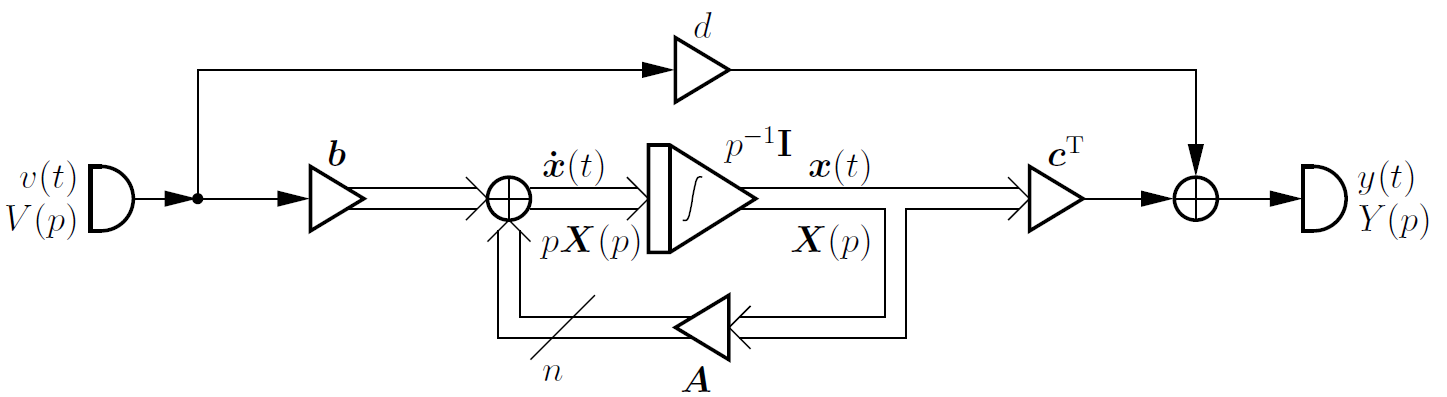
\includegraphics[width=1\textwidth]{images_ssp/Zustandsraumreal}\\
			%	\vspace{0.5 cm}
		\end{minipage}
	\end{itemize}
\end{infobox}



\section{Zeitkontinuierliche Systeme}
\subsection*{Zustandsraumdarstellung \footnotesize{(SISO-LTI-System)}}

	\begin{tabular}{ll}
	Zustandsgleichung: & $ \dot{\vec x}(t) = \ma A \vec x(t) + \vec b v(t) $\\
	Ausgangsgleichung: & $ y(t) = \vec c^{\ma T} \vec x(t) + d v(t)$ \\\\
	Zustandsvektor & $\vec x(t) \in \mathbb R^n$ \\
	Ausgangssignal & $ y(t) \in \mathbb R$ \\
	Eingangssignal: & $ v(t) \in \mathbb R$ \\
	Zustandsmatrix & $\ma A\in \mathbb R^{n \times n}$ \\
	Einkoppelvektor & $\vec b \in \mathbb R^{n}$ \\
	Auskoppelvektor & $\vec c \in \mathbb R^{n}$ \\
	Durchgriff & $d \in \mathbb R$ \\

\end{tabular}

\subsection*{Systemantworten}
\ul{Annahme:} Alle $n$ Eigenwerte von $\ma A$ sind verschieden.\\

%Zero-state, Steady-state, Impulsantwort
\textit{Lösung der Zustandsgleichung} (für $t \ge t_0$):\\
$\vec x (t) =  \vec x_{\textmd{zero-input}}(t) + \vec x_{\textmd{zero-state}}(t)$ \\
$= \textmd{exp}(\ma A (t-t_0)) \vec x (t_0) + \int\limits_{t_0}^t \textmd{exp}(\ma A(t-t')) \vec b \vec v(t') \mathrm{d}t'$\\

Einsetzen der Lösung von $\vec x(t)$ in die Ausgangsgleichung liefert (mit $t_0 = 0$):\\
$y(t) = y_{\textmd{zero-input}}(t) + y_{\textmd{zero-state}}(t)$\\
$y_{\textmd{zero-input}}(t) = \ma{c^T} \textmd{exp}(\ma A t) \vec x (0) = \sum\limits_{i=1}^{n} \textmd{exp}(\lambda_i t) y_{0i}$\\
$y_{\textmd{zero-state}}(t) = (h*v)(t)$\\

mit $h(t)$: Impulsantwort\\
$\boxed{h(t) = \vec c^{\ma T} \textmd{exp}(\ma A t) \vec b + d\delta(t)}$\\

Damit das System stabil ist, muss gelten: $\forall i : \lambda_i < 0$\\

\subsection*{Übertragungsfunktion}
$H(p) = \frac{Y(p)}{V(p)} = \ma{c}^T (p\ma{I} - \ma{A})^{-1} \ma{b} + d = \mathcal{L}\{h(t)\}$\\
%$(p \ma{I} - \ma{A})^{-1} = \frac{adj(p\ma{I} - \ma{A})}{\det(p\ma{I} - \ma{A})}$ \\\\

$\Rightarrow \boxed{H(p) = \dfrac{\beta_0 p^n + \beta_1 p^{n-1} + \dots + \beta_{n-1} p + \beta_n}{p^n + \alpha_1 p^{n-1} + \dots + \alpha_{n-1} p + \alpha_n}}$ \\

mit $\beta_0 = d$\\
System ist kausal $\Leftrightarrow$ Zählergrad $\le$ Nennergrad.\\
Die Pole der Übertragungsfunktion entsprechen den Eigenwerten des Systems: $p_{\infty,i} = \lambda_i$
\subsection*{Realisierungsformen}
\subsubsection*{Parallelform}

Transformation des Systems in Normalform liefert folgende Zustandsraumdarstellung:\\
$ \dot{\vec \xi}(t) = \ma \Lambda \vec \xi(t) + \vec \mu v(t) $\\
$ y(t) = \vec \eta^{\ma T} \vec \xi(t) + d v(t)$ \\

mit EVD $\ma A = \ma Q \ma \Lambda \ma Q ^{-1}$, $\vec \mu = \ma Q ^{-1} \vec b$, $\vec \eta^{\ma T} = \vec c ^{\ma T} \ma Q$ und $\vec \xi(t) = \ma Q ^{-1} \vec x(t)$, wobei $\ma Q = \mat{\vec q_1, \dots, \vec q_n}$ (Matrix der Eigenvektoren) und $\ma \Lambda = \textmd{diag}(\lambda_1,\dots,\lambda_n)$.\\


Daraus ergibt sich:\\
$H(p) = \vec \eta^T (p\ma{I} - \ma{\Lambda})^{-1} \vec \mu + d$
$ = d +\sum\limits_{i=1}^{n}\eta_i \dfrac{\mu_i}{p-\lambda_i}$\\
$ = d + \sum\limits_{i=1}^{n} H_i(p)$\\

\begin{minipage}[h]{0.5\textwidth}
	%\vspace{0.1 cm}
	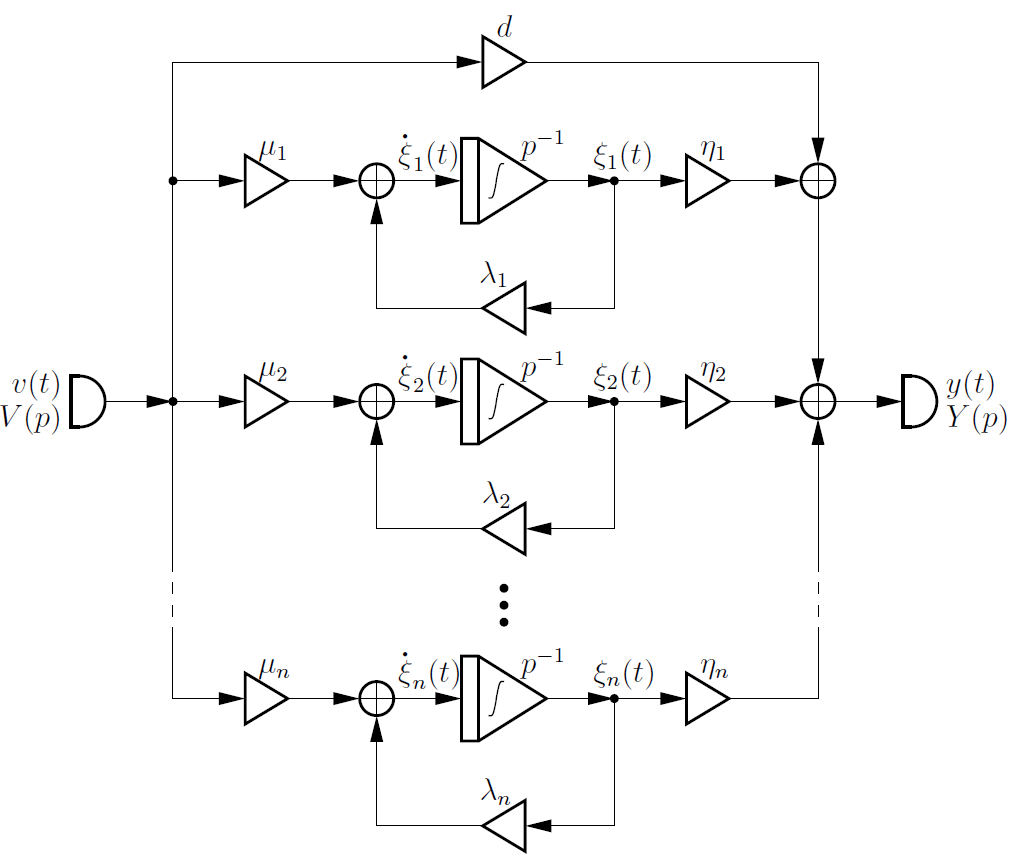
\includegraphics[width=0.56\textwidth]{images_ssp/Parallelform}\\
	%	\vspace{0.5 cm}
\end{minipage}
\newpage
Falls  $H(p)$  gegeben:\\
mittels Partialbruchzerlegung $H(p)$ auf die obige Form bringen!
\begin{cookbox}{Partialbruchzerlegung von $H(p)$}
	\begin{itemize}
		\item[1)] Falls Zählergrad = Nennergrad:\\ Polynomdivison. Konstanter Term = $d$
		\item[2)] Nenner von $H(p)$ in Faktoren zerlegen\\
		Für reelwertige Pole $p_{\infty,i}$ von $H(p)$:\\
		$H_i(p) = \dfrac{A_i}{p - p_{\infty,i}}$\\
		Für konjugiertkomplexes Polpaar $p_{\infty,2} = p_{\infty,i}^*$ von $H(p)$:\\
		$H_i^{(2)}(p) = \dfrac{A p + B}{p^2 - 2 \textmd{Re}{\{p_{\infty,1}\}}p + |p_{\infty,1}|^2}$
		\item[3)] Nenner ausmultiplizieren, Koeffizienten $A_i$ bestimmen:
		Koeffizientenvergleich oder Pole für $p$ einsetzen
		\item[4)] $\mu_i = A_i$, $\eta_i = 1$ in obenstehenden Signalflussplan einsetzen
	\end{itemize}
ACHTUNG: Realisierungsstruktur für $H_i^{(2)}(p)$ ist nicht eingezeichnet!\\
Realisierung z.B. mit Beobachter/Steuerernormalform.
	
\end{cookbox}


\subsubsection*{Kaskadenform}
Zerlegt man Zähler und Nenner von $H(p)$ in Faktoren, erhält man:\\

$H(p) = \beta_0 \dfrac{\prod_{k=1}^{n}(p-p_{0,k})}{\prod_{k=1}^{n}(p - p_{\infty,i})} = \prod\limits_{k=1}^{n}H_i(p)$\\

wobei $p_{0,i}$ = Nullstellen, $p_{\infty,i}$ = Pole.
\\\\
\begin{minipage}[t]{0.6\textwidth}
	%	\vspace{0.3 cm}
	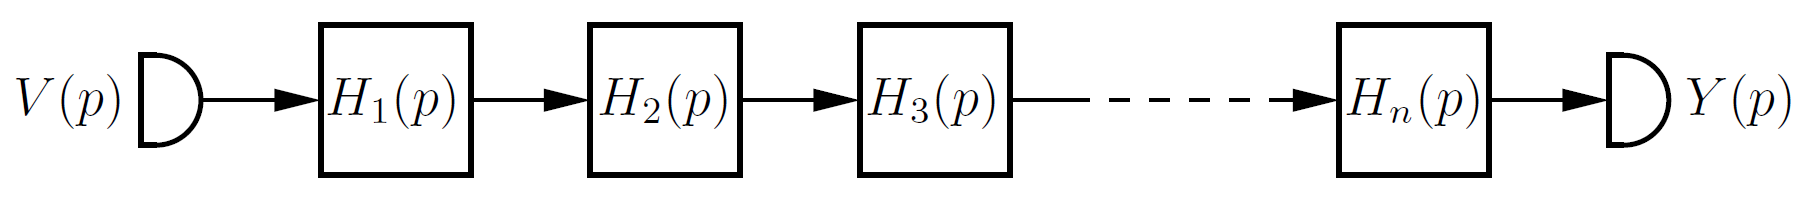
\includegraphics[width=0.5\textwidth]{images_ssp/Kaskadenform}\\
	%	\vspace{0.5 cm}
\end{minipage}
\\\\
\begin{cookbox}{Faktorzerlegung von $H(p)$}
	\begin{itemize}
		\item[1)] Nenner und Zähler von $H(p)$ in Faktoren zerlegen
		\item[2)] Aufteilen der Faktoren in folgende Form:\\
		$H_i^{(1)}(p) = \dfrac{\beta_{0,i} p + \beta_{1,i}}{p + \alpha_{1,i}}$, bzw. \\
		$H_i^{(2)}(p) = \dfrac{\beta_{0,i} p^2 + \beta_{1,i} p + \beta_{2,i}}{p + \alpha_{1,i} p + \alpha_{2,i}}$ für konjugiertkomplexe Polpaare \\
		\item[3)] Teilübertragungsfunktionen einzeln realisieren und in Serie verbinden
	\end{itemize}
ACHTUNG: Teilübertragungsfunktion muss kausal sein (Nennergrad $\ge$ Zählergrad)\\
\end{cookbox}


\subsubsection*{Kanonische Steuererform}
Aus den Koeffizienten von $H(p)$ in der Form:\\

$H(p) = \dfrac{\beta_0 p^n + \beta_1 p^{n-1} + \dots + \beta_{n-1} p + \beta_n}{p^n + \alpha_1 p^{n-1} + \dots + \alpha_{n-1} p + \alpha_n} $\\

kann man direkt folgende Realisierung aufstellen:\\\\
\begin{minipage}[t]{0.6\textwidth}
	%	\vspace{0.3 cm}
	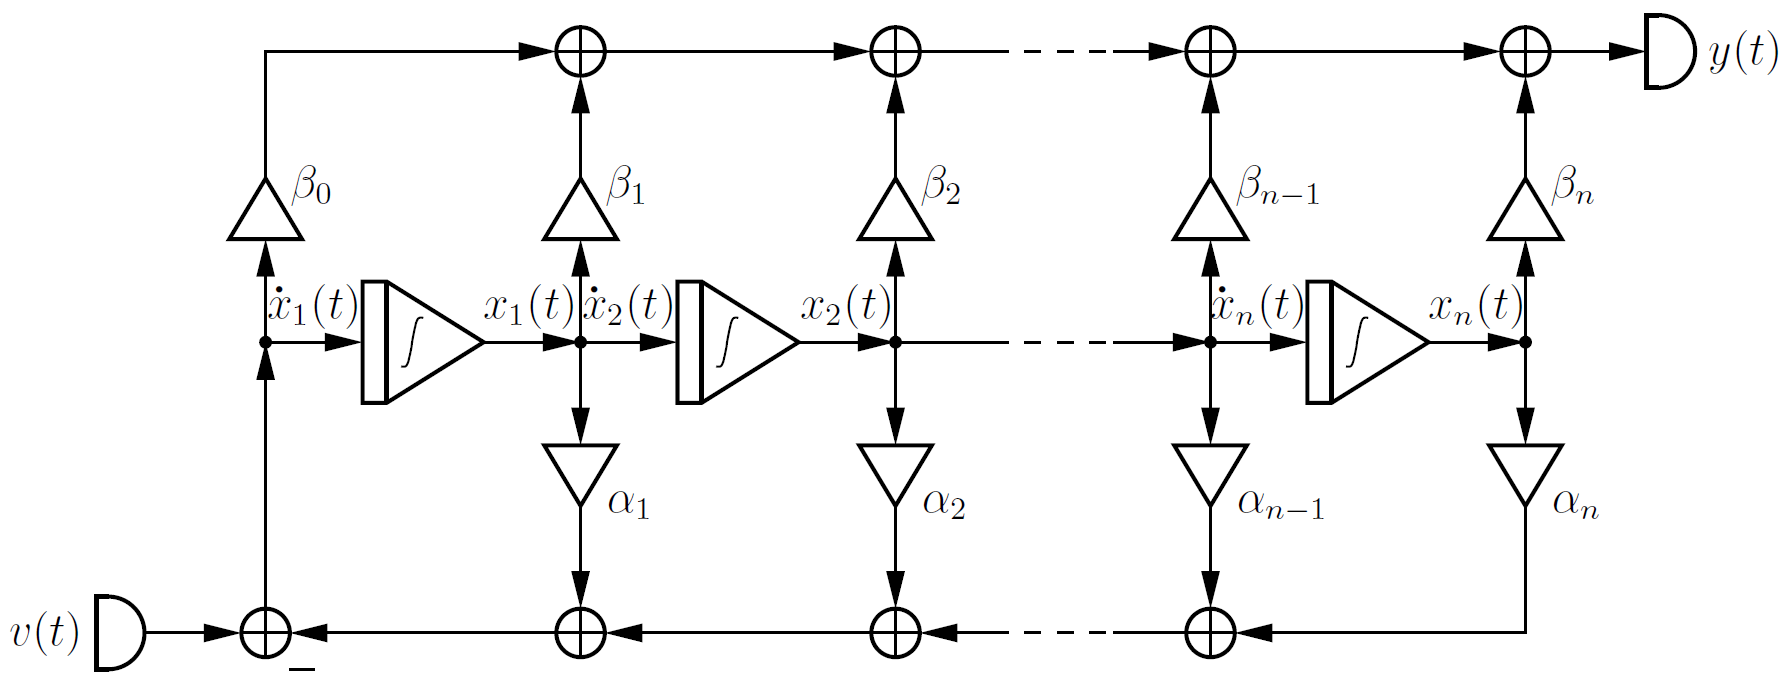
\includegraphics[width=0.5\textwidth]{images_ssp/Steuererform}\\
%	\vspace{0.5 cm}
\end{minipage}

\subsubsection*{Kanonische Beobachterform}
Die Beobachterform ist die Transponierte der Steuererform und lässt sich somit gleich aufstellen.

\begin{minipage}[t]{0.6\textwidth}
	%	\vspace{0.3 cm}
	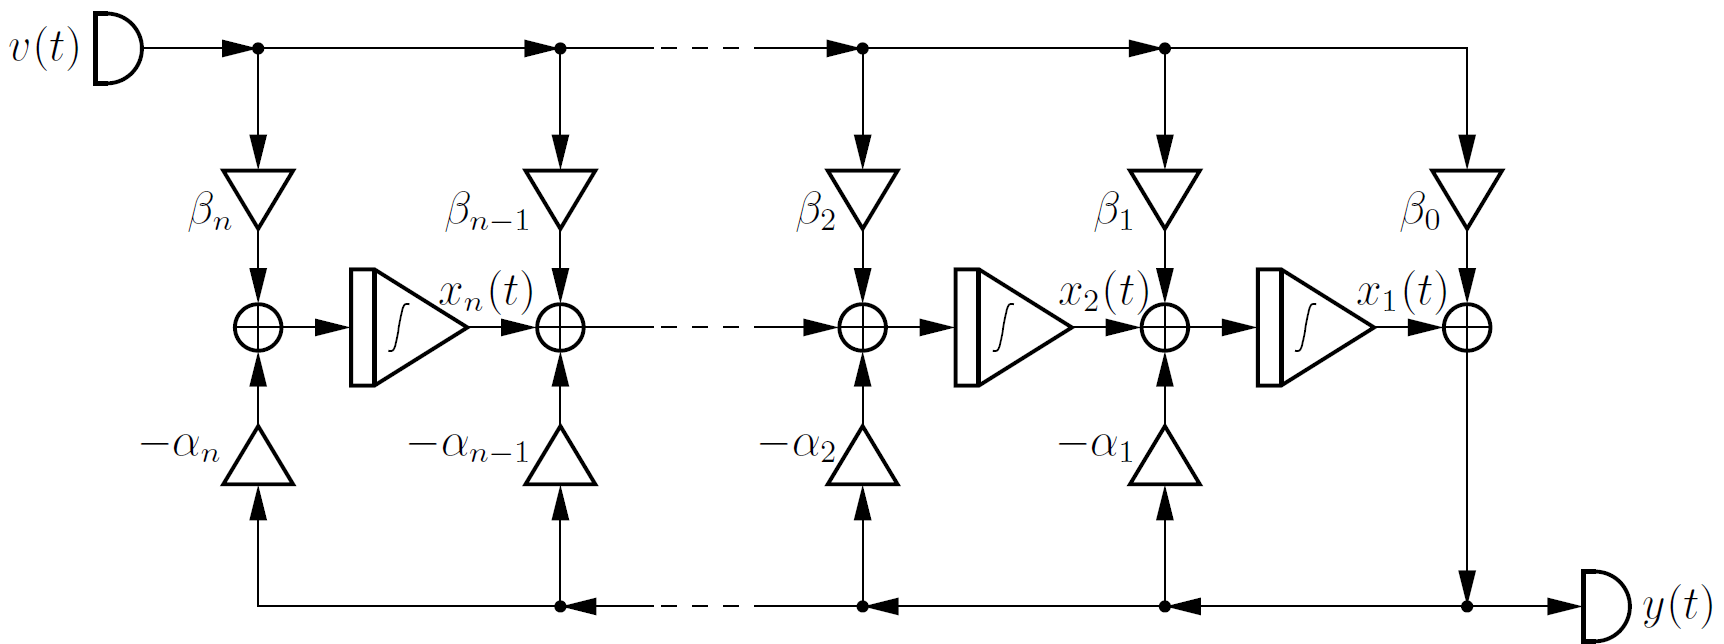
\includegraphics[width=0.5\textwidth]{images_ssp/Beobachterform}\\
%	\vspace{0.5 cm}
\end{minipage}

%\subsubsection*{Verlustloser Prototyp}
%\begin{minipage}[t]{0.6\textwidth}
	%	\vspace{0.3 cm}
%	\includegraphics[width=0.5\textwidth]{images_ssp/lossless_prototyp}\\
	%	\vspace{0.5 cm}
%\end{minipage}

\subsubsection*{Sensitivität}
Die Sensitivität eines Systems bezogen auf Parameterabweichungen ist die Rate der Abweichung der erwünschten Eigenschaft (z.B. Betrag der Übertragungsfunktion) zum nominalen Wert, verursuacht durch beispielsweise ungenauen Parameterwerten. Die Kanonischen Formen weisen die schlechteste Sensitivität vor, gefolgt von der Parallelform und Kaskadenform. Der verlustlose Prototyp ist am robustesten gegenüber Parameterabweichungen.

\subsection*{Standardapproximationen / Filtersynthese}
Diverse Standardapproximationen sind als Tiefpass n-ter Ordnung mit folgender Übertragungsfunktion gegeben:\\

$H(p)=\dfrac{1}{p^n + \alpha_1 p^{n-1} + \dots + \alpha_{n-1} p + \Omega_{\textmd{passband}}^n}$\\

mit normalisierter cut-off-Frequenz $\Omega_{\textmd{passband}} = 1$.\\
Die Umwandlung zu willkürlichen cut-off-Frequenzen erfolgt mit: $p \rightarrow \frac{p}{\omega_{\textmd{passband}}}$\\ %omega = 2 pi f
Für andere Filtertypen wendet man folgende Transformation an:
\begin{itemize}
	\item Hochpass: $p \rightarrow \frac{1}{p}$
	\item Bandpass: $p \rightarrow a(p + \frac{1}{p})$
	\item Bandsperre: $p \rightarrow (a(p + \frac{1}{p}))^{-1}$
\end{itemize}
mit Parameter $a = \frac{1}{\textmd{Bandweite}}$\\
Für technische Frequenzen ersetzt man $p \rightarrow j\omega$\\

Je nach gewünschtem Verhalten des Frequenzgangs nimmt man die entsprechenden Koeffizienten des Nennerpolynoms aus einer Filtertabelle. 

\subsubsection*{Butterworth Filter}
Eigenschaft: maximal flach im Passband

\subsubsection*{Chebyshev Filter}
Eigenschaft: Abweichung von $|H(j\omega)|$ zum gewünschten Wert ist im Passband minimiert:\\
$\min\limits_{\alpha_i} \max\limits_{\omega \in [0,\omega_{\textmd{cut-off}}]}||H(j\omega)| - 1|$ \\
Daraus folgt konstante Welligkeit (equiripple) im Passband.
%Daraus folgt ein equiripple-Verhalten.
%konstante Welligkeit
\subsubsection*{Cauer Filter}
Eigenschaft: konstante Welligkeit (equiripple) im Passband und Stoppband

\subsubsection*{Bessel Filter}
Eigenschaft: möglichst linearer Phasenverlauf im Passband.
Das bedeutet: möglichst konstante Gruppenlaufzeit. Wichtig für Systeme mit Frequenz- und Phasenmodulation.
%-----------------------------------------------------------------------------------------------------

\section{Zeitdiskrete Systeme}
\subsection*{Zustandsraumdarstellung \footnotesize{(SISO-LTI-System)}}
\begin{tabular}{ll}
	Zustandsgleichung: & $ \vec x[k+1] = \ma A \vec x[k] + \vec b v[k] $\\
	Ausgangsgleichung: & $ y[k] = \vec c^{\ma T} \vec x[k] + d v[k]$ \\	
\end{tabular}

\subsection*{Systemantworten}
\ul{Annahme:} Alle n Eigenwerte von $\ma A$ sind verschieden.\\

\textit{Lösung der Zustandsgleichung} (für $t \ge 0$, $t_0 = 0$):\\\\
$\vec x [k] =  \vec x_{\textmd{zero-input}}[k] + \vec x_{\textmd{zero-state}}[k]$ \newline
$= \ma A^k \vec x [0] + \sum\limits_{i=0}^{k-1} \ma A^{k-1-i} \vec b \vec v[i]$

Einsetzen der Lösung von $\vec x(t)$ in die Ausgangsgleichung liefert:\newline

$y[k] = y_{\textmd{zero-input}}[k] + y_{\textmd{zero-state}}[k]$\newline

$y_{\textmd{zero-input}}[k] = \ma{c^T} \ma A^k \vec x [0] = \sum\limits_{i=1}^{n} \lambda_i^k y_{0i}$\newline

$y_{\textmd{zero-state}}[k] = (h*v)[k]$\\

mit $h[k]$: Impulsantwort\\
$\boxed{h[k] = \sum\limits_{i=1}^\infty \vec c^{\ma T} \ma A^{i-1} \vec b \delta[k-i] + d\delta[k]}$\\

Damit das System stabil ist, muss gelten: $\forall i : |\lambda_i| < 1$

\subsection*{Übertragungsfunktion}
$H(z) = \frac{Y(z)}{V(z)} = \ma{c}^T (z\ma{I} - \ma{A})^{-1} \ma{b} + d = \mathcal{Z}\{h[k]\}$\\

$\boxed{H(z) = \dfrac{\beta_0 z^n + \beta_1 z^{n-1} + \dots + \beta_{n-1} z + \beta_n}{z^n + \alpha_1 z^{n-1} + \dots + \alpha_{n-1} z + \alpha_n}}$ \\\\

Zähler und Nenner durch $z^n$ teilen:\\

$\boxed{H(z) = \dfrac{\sum_{i=0}^n \beta_i z^{-i}}{1 + \sum_{i=1}^n \alpha_i z^{-i}}}$ \tab mit $\beta_0 = d$\\

\ul{Zusammenhang $p$ und $z$:} $\boxed{z= e^{pT}}$\\

Nach Rücktransformation in Zeitbereich erhält man die Differenzengleichung:\\
$y[k] + \sum\limits_{i=1}^n \alpha_i y[k-i] = \sum\limits_{i=0}^n \beta_i v[k-i]$\\

System ist kausal $\Leftrightarrow$ Zählergrad $\le$ Nennergrad.

\subsubsection*{Realisierungsformen}
Zur Realisierung der Übertragungsfunktion diskreter Systeme können dieselben Methoden wie bei zeitkontinuierlichen Systemen angewandt werden. Für zeitdiskrete Systeme sehen Beobachterform (links) und Steuererform (rechts) wie folgt aus:

\begin{minipage}[t]{0.6\textwidth}
	%	\vspace{0.3 cm}
	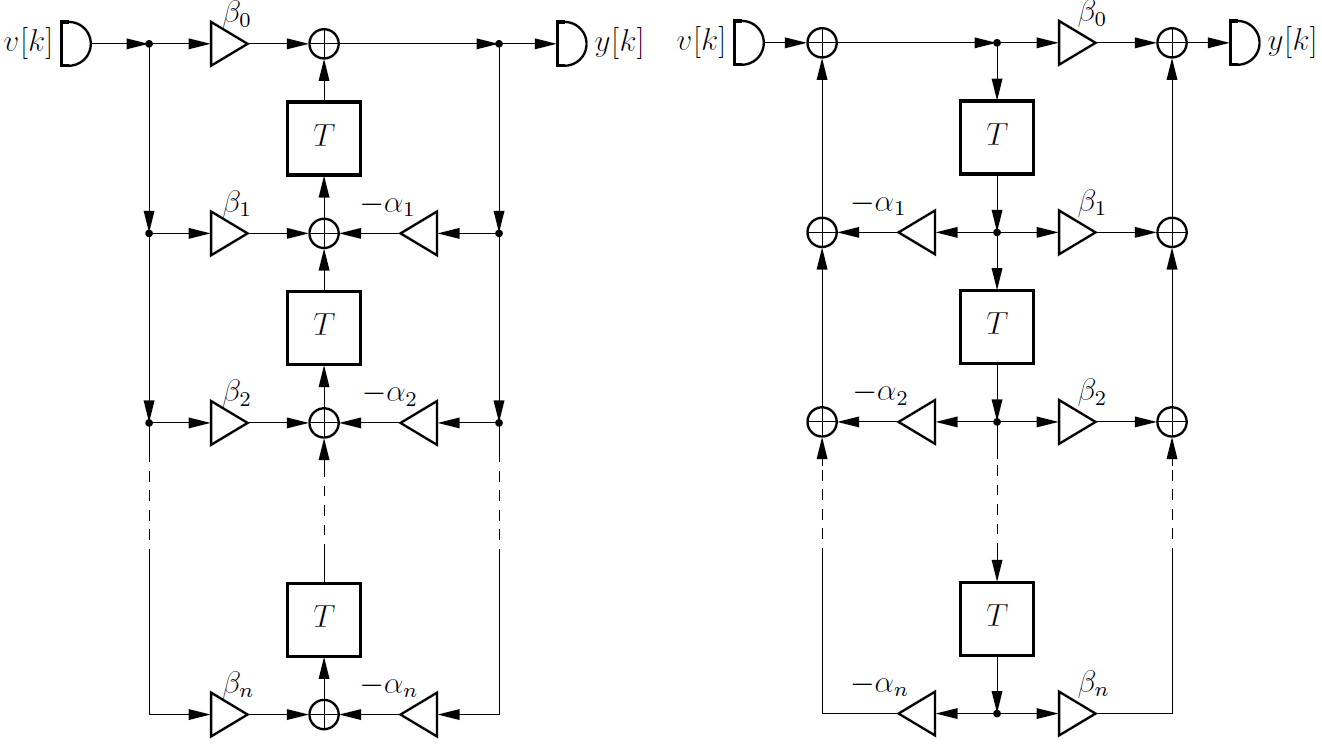
\includegraphics[width=0.5\textwidth]{images_ssp/DigSys_kanonische}\\
	%	\vspace{0.5 cm}
\end{minipage}
\subsection*{Anwendung zeitdiskreter Systeme auf analoge Signale}
\begin{minipage}[t]{0.6\textwidth}
	%	\vspace{0.3 cm}
	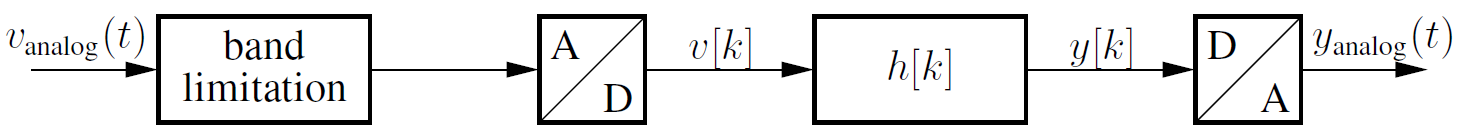
\includegraphics[width=0.5\textwidth]{images_ssp/DigSys_in_anaSys}\\
	%	\vspace{0.5 cm}
\end{minipage}
Um ein zeitkontinuierliches (analoges) Signal mit einem digitalen Filter zu bearbeiten, muss vorerst eine Bandlimitierung vorgenommen werden, damit es zu keinen Interferenzen im Spektrum (Aliasing) des gesampelten Signals $v[k]$ kommt. Außerdem ist die Bandlimitation nach dem Nyquist-Kriterium notwendig, um aus dem digitalen Signal $y[k]$ das analoge Signal $y_{analog}$ korrekt rekonstruieren zu können.\\

$H_{\textmd{analog}}(j\omega) = \dfrac{Y_{\textmd{analog}}(j\omega)}{V_{\textmd{analog}}(j\omega)} = H(z=e^{j\omega T})$\\

$W_{\textmd{sampled}}(j\omega) = \mathcal{F}\{w(t)\sum\limits_{i=-\infty}^{\infty}\delta(t-iT)\} \\ \tab = \sum\limits_{l=-\infty}^{\infty}W(j(\omega - l\frac{2\pi}{T}))$\\

mit $f_s = \frac{1}{T} =$ Samplingfrequenz

\subsection*{FIR-Systeme \footnotesize{(Finite Impulse Response)}}
Systeme mit einer Impulsantwort endlicher Länge werden realisiert, indem in der Differenzengleichung keine rekursiven Terme enthalten sind $\rightarrow \forall i : \alpha_i = 0$.\\

$y[k] = \sum\limits_{i=0}^n \beta_i v[k-i]$\\
$H(z) = \sum\limits_{i=0}^n \beta_i z^{-i} = \dfrac{\sum_{i=0}^n \beta_i z^{n-i}}{z^n}$\\

Es gilt $\forall i: z_{\infty,i} = 0$, somit sind FIR-Systeme immer stabil.

\begin{minipage}[t]{0.6\textwidth}
	%	\vspace{0.3 cm}
	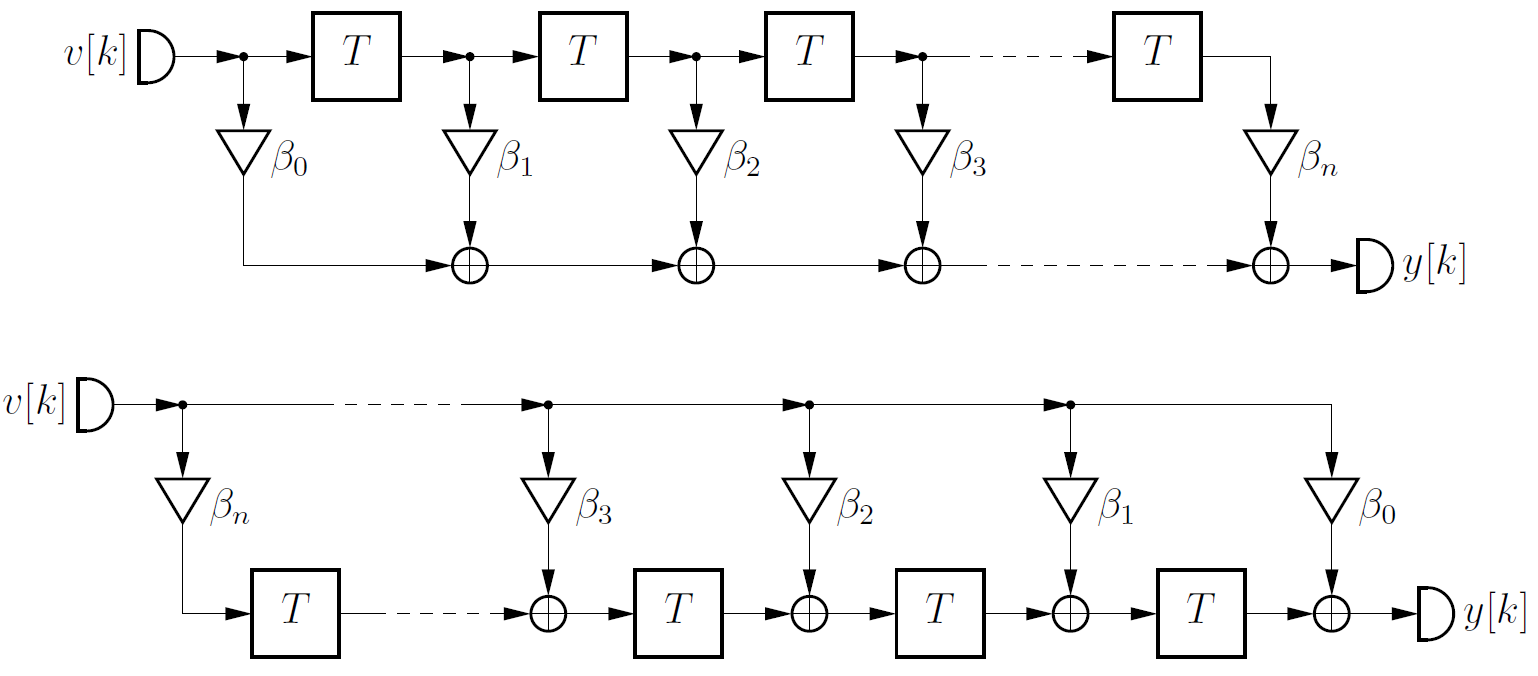
\includegraphics[width=0.5\textwidth]{images_ssp/FIR_Realisierung}\\
	%	\vspace{0.5 cm}
\end{minipage}
\subsection*{FIR-Filter Design}
Vorteile von FIR-Filter:\\Einfache Implementierung; immer stabil.
\subsubsection*{Fensterung}
Idee: Samplen einer Impulsantwort mit unendlicher Dauer für ein endliches Zeitfenster $[-T,T]$, bzw. $[0,T]$.
Häufige Wahl der Fensterfunktion:\\

$w[k] = a - b \cos(\frac{\pi}{N}(k+N)) + c \cos(\frac{2\pi}{N}(k+N)) \\ \text{für } -N \le k \le N, \tab 0 \text{ sonst}$\\

\begin{tabular}{|c|c|c|c|}
	\hline
	 Fensterfunktion & a & b & c \\
	\hline
	Rechteck & 1 & 0 & 0 \\
	\hline
	Hanning & 0.5 & 0.5 & 0 \\
	\hline
	Hamming & 0.54 & 0.56 & 0 \\
	\hline
	Blackman & 0.42 & 0.5 & 0.08 \\
	\hline
\end{tabular}
\\

Beispielsweise hat die Hanning-Fensterung ein besseres Verhalten des Frequenzgangs im Stoppband als mit Rechteckfensterung zur Folge, jedoch auch eine schlechtere Unterdrückung der Intersymbolinterferenz.

\subsubsection*{Linearphasige FIR-Filter}
 Es gilt für $H(z)$ mit $z=e^{j\omega T}$:
\begin{itemize}
	\item $n$ ungerade, $N = \frac{n-1}{2}$, $\beta_i = \beta_{n-i}$:\\
	$H(e^{j\omega T}) = e^{-j\omega\frac{n}{2}T} \sum\limits_{i=0}^{N} 2\beta_i \cos((\frac{n}{2}-i)\omega T)$
	\item $n$ gerade, $N = \frac{n}{2}-1$, $\beta_i = \beta_{n-i}$:\\
	$H(e^{j\omega T}) = e^{-j\omega\frac{n}{2}T} \big(\beta_{n/2} + \sum\limits_{i=0}^{N} 2\beta_i \cos((\frac{n}{2}-i)\omega T)\big)$
	\item $n$ ungerade, $N = \frac{n-1}{2}$, $\beta_i = -\beta_{n-i}$:\\
	$H(e^{j\omega T}) = e^{j(-\omega\frac{n}{2}T + \frac{\pi}{2})} \sum\limits_{i=0}^{N} 2\beta_i \sin((\frac{n}{2}-i)\omega T)$
	\item $n$ gerade, $N = \frac{n}{2}-1$, $\beta_i = -\beta_{n-i}$, $\beta_{n/2} = 0$:\\
	$H(e^{j\omega T}) = e^{j(-\omega\frac{n}{2}T + \frac{\pi}{2})} \sum\limits_{i=0}^{N} 2\beta_i \sin((\frac{n}{2}-i)\omega T)$
\end{itemize}

Somit tragen für Filter mit gerade- oder ungerade symmetrischen Koeffizienten nur die Terme \\
$e^{j\varphi (\omega)} = e^{j(-\omega\frac{n}{2}T)}$, bzw. $e^{j\varphi (\omega)} = e^{j(-\omega\frac{n}{2}T + \frac{\pi}{2})}$ \\ 
zur Phase bei, was für alle vier Fälle dieselbe konstante Gruppenlaufzeit zur Folge hat:\\

\tab \tab $\boxed{\tau_{gr} = - \diff{\varphi(\omega)}{\omega} = \frac{nT}{2}}$.\\

Effiziente Implementierung ($n$ ungerade, $\beta_i = \beta_{n-i}$):\\
\begin{minipage}[t]{0.6\textwidth}
	%	\vspace{0.3 cm}
	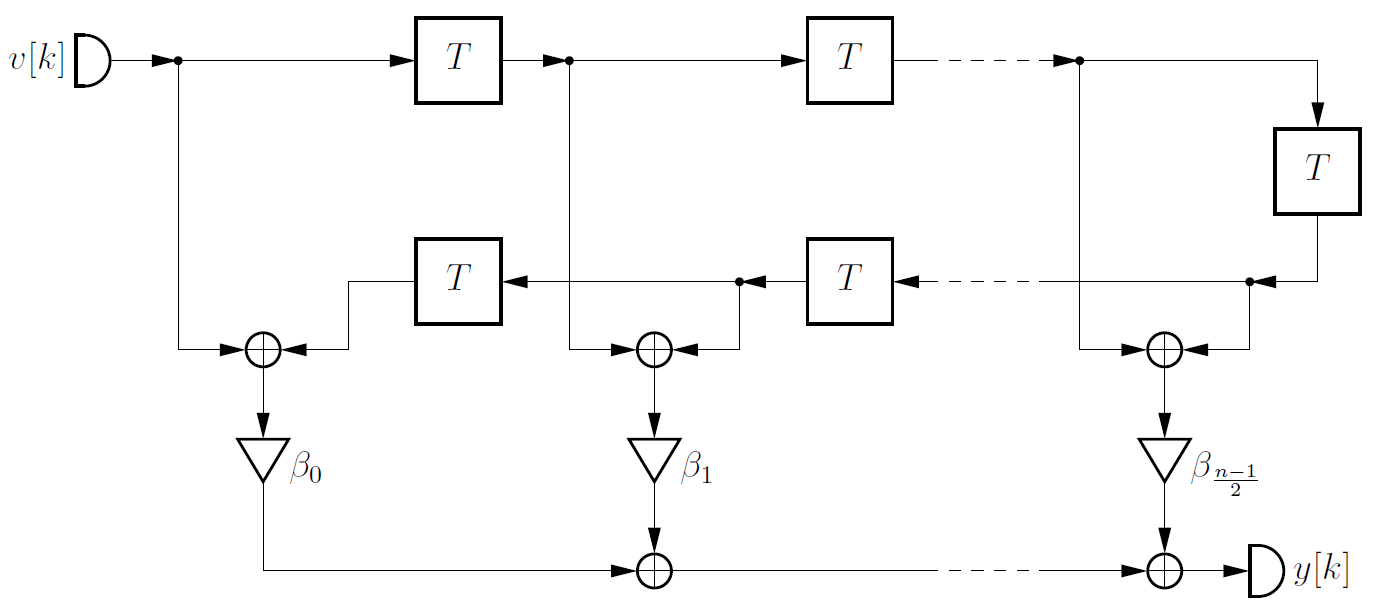
\includegraphics[width=0.5\textwidth]{images_ssp/FIR_linPha}\\
	%	\vspace{0.5 cm}
\end{minipage}
\subsubsection*{Anforderungen an Frequenzgang linearphasiger FIR-Filter stellen}
\underline{1. Least Squares Methode}\\
Die LS-Methode liefert die optimalen Koeffizienten $\beta_i$, für denen der Filter gegebene Anforderungen am Frequenzgang erfüllt bzw. approximiert.
Der Vektor $\vec s$ enthält alle $M$ Anforderungen:\\
$\vec s = [H'(\omega_1), \dots , H'(\omega_M)]$
mit $H'(\omega_m) = |H(e^{j\omega T})|$.\\
Beispiel für $n$ ungerade, $\beta_i = \beta_{n-i}$:\\
$H'(\omega) = \sum\limits_{i=0}^{N} 2\beta_i \cos((\frac{n}{2}-i)\omega T)$, $\Rightarrow$\\

$\vec t(\omega_k) = [2\cos((\frac{n}{2})\omega_k T), 2\cos((\frac{n}{2} - 1)\omega_k T) , \dots , 2\cos((\frac{1}{2})\omega_k T)]^{\ma T}$

$\vec \theta = [\beta_0, \beta_1, \dots , \beta_N]$\\

Somit lassen sich die Anforderungen wie folgt formulieren:\\
\tab $\ma T \vec \theta = \vec s$ \tab mit $\ma T = \mat{\vec t^{\ma T}(\omega_1) \\ \vec t^{\ma T}(\omega_2) \\ \vdots \\ \vec t^{\ma T}(\omega_M)} \in \mathbb{R}^{M \times N+1}$

\begin{itemize}
	\item $M = N+1$: quadratisches $\ma T$\\
	eindeutig lösbares Gleichungssystem. $ \Rightarrow \vec \theta = \ma T^{-1} \vec s$
	\item $M > N+1$: langes $\ma T$\\
	überbestimmtes Gleichungssystem ($n < 2M-1 $). Näherungslösung: 
	$\vec \theta_{LS} = (\ma T^{\ma T} \ma T)^{-1} \ma T ^{ \ma T} \vec s$
	\item $M < N+1$: breites $\ma T$\\
	unterbestimmtes Gleichungssystem. Lagragne-Ansatz liefert: 
	$\vec \theta_{LS} = \ma T ^{ \ma T}(\ma T \ma T ^{ \ma T})^{-1} \vec s$ 
\end{itemize}

\underline{2. Remez Algorithmus}\\
Der Remez Algorithmus liefert die optimalen Koeffizienten $\beta_i$, falls man als Anforderung am Filter ein minimax-Problem (Chebyshev / Cauer Designtyp) stellt.\\

$\vec \theta_{opt} = \min\limits_{\vec \theta} \max\limits_{\omega \in [0,\frac{\pi}{T}]} | W(\omega)(H'(\omega) - D(\omega))|$\\

Somit wird der gewichtete maximale Fehler minimiert. Üblich wählt man:\\

$D(\omega) = \left\{
\begin{array}{ll}
1 & \quad 0 \le \omega \le \omega_0 \\
0 & \quad  \omega_0 < \omega \le \frac{\pi}{T} \\
\end{array} \right.
$ mit $\omega_{\text{pass}} < \omega_0 < \omega_{\text{stop}}$\\

$W(\omega) = \left\{
\begin{array}{cl}
W_p & \quad 0 \le \omega \le \omega_{\text{pass}} \\
0 & \quad  \omega_{\text{pass}} < \omega < \omega_{\text{stop}} \\
W_s & \quad \omega_{\text{stop}} \le \omega \le \frac{\pi}{T}
\end{array} \right.
$\\

%Remez-Algorithm einfügen? n-1/2 = N, n grad system
Eigenschaften von $\Gamma(\omega) = W(\omega)(H'(\omega) - D(\omega))$):\\($N=\frac{n-1}{2}$ mit $n$: Grad des Systems)
	\begin{itemize}
		\item $|\Gamma(\omega)|$ hat $N+2$ Maxima im Intervall $\Omega \in [0,\frac{\pi}{T}]$
		\item Alle Maxima haben den selben Wert $|\Gamma(\omega_i)| = ||\Gamma(\omega)||_{\infty}$
		\item $\Gamma(\omega_i) = -\Gamma(\omega_{i+1})$
	\end{itemize}

\subsubsection*{Minimalphasige FIR-Filter}
Die Übertragungsfunktion eines FIR-Filters lässt sich wie folgt schreiben:\\
$H(z) = \sum\limits_{i=0}^n \beta_i z^{-i} = z^{-n} \beta_0 \prod\limits_{i=1}^n (z-z_i) $\\
Um die Gruppenlaufzeit zu minimieren, führt man folgende Substitution durch:\\

$\forall i$ mit $|z_i| > 1$: ersetze $z_i \rightarrow \dfrac{1}{z_i^*} = \dfrac{z_i}{|z_i|^2}$\\

Dies entspricht einer Kaskadierung mit einem Allpass folgender Form:\\
$H_{\text{AP}}(z) = |z_i|\dfrac{z-1/z_i^*}{z-z_i}$, mit $|H_{\text{AP}}(z)| = 1$.\\

Die Gruppenlaufzeit wird somit pro Substitution um \\

$\tau_{gr,i} = -T\dfrac{|z_i|^2 - 1}{|z_i|^2 - 2|z_i|\cos(\omega T-\phi_i) + 1} < 0$ \\

verkürzt, ohne den Amplitudengang zu verändern ($\phi_i = \arg(z_i)$).

Der Allpass $H_{\text{AP}}(z)$ ist aufgrund der Polstelle $|z_i| > 1$ nicht stabil und somit nicht realisierbar, jedoch die Kaskadierung von Allpass und $H(z)$ aufgrund von Pol-Nullstellen-Kompensation ist realisierbar.

\subsection*{IIR-Systeme \footnotesize{(Infinite Impulse Response)}}
Für irgendein $\alpha_i \neq 0$ wird die Impulsantwortdauer unendlich lang.
\subsection*{IIR-Filter Design}
Man definiert die Frequenzvariable $\psi(z)$ so, dass der Imaginäranteil von $p$ auf das Intervall $j[-\frac{T}{2}, \frac{T}{2}]$ abgebildet wird. Somit lassen sich die Eigenschaften der Standardapproximationen zeitkontinuierlicher Systeme mit einfacher Substitution von $p$ mit $\psi(z)$ in $H(p)$ auf zeitdiskrete Systeme übertragen:\\

$\psi = \text{tanh}(\frac{pT}{2}) = \frac{z-1}{z+1}$ \tab ($\leftarrow$ Bilineartransformation)\\

$z = \frac{1+\psi}{1-\psi} = e^{pT}$\\

$p = \frac{2}{T}\text{artanh}(\psi) = \frac{1}{T}\ln(z)$\\

$\rightarrow$ Mit $\psi= \epsilon + j\varphi$ und $p = \sigma + j\omega$:\\
$\varphi = \tan(\frac{\omega T}{2})$ \tab $\omega = \frac{2}{T}\arctan(\varphi)$\\

\begin{cookbox}{Zeitdiskrete Filter nach Standardappr. }
	\begin{itemize}
		\item[1)] Berechne $\varphi_{\textmd{passband}}$ aus $\omega_{\textmd{passband}}$
		\item[2)] Entnehme der Tabelle der gewünschten Standardapproximation die Koeffizienten der Polynome für Zähler und Nenner und entferne die Normalisierung mit $\varphi_{\textmd{cut-off}}$
		\item[3)] Wähle die Realisierungsstruktur
		\item[4)] Entweder a) oder b):\\
		a) Setze $p \leftarrow \psi = \frac{z-1}{z+1}$ in $H(p)$ der Filterapproximation und berechne die neuen Koeffizienten der Polynome in Zähler und Nenner von $H(z)$\\
		b) Ersetze die Integratoren ($H(p) = \frac{1}{\alpha p}$) der zeitkontinuierlichen Realisierung mit folgender Struktur ($H(z) = \frac{1}{\alpha}\frac{1+z^{-1}}{1-z^{-1}}$):
	\end{itemize}
\end{cookbox}
\begin{minipage}[t]{0.5\textwidth}
	%\vspace{0.1 cm}
	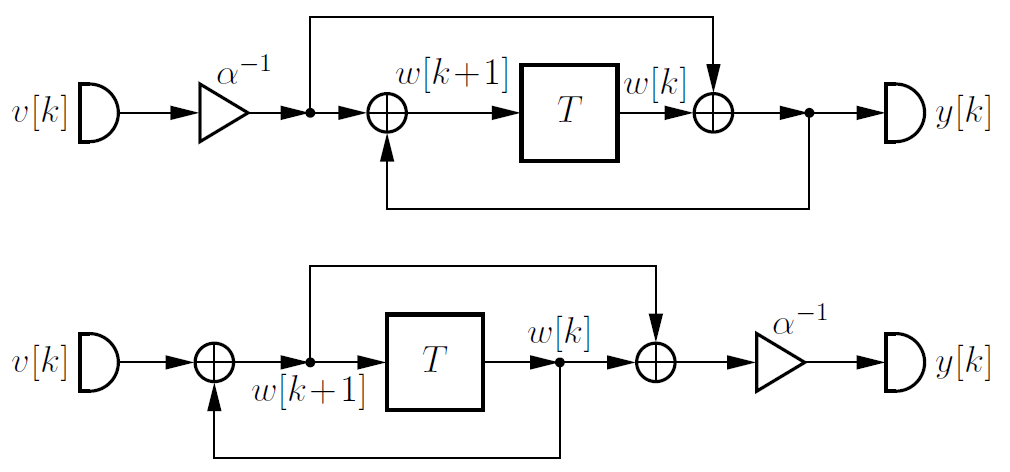
\includegraphics[width=0.6\textwidth]{images_ssp/Zeitdisk_Int}\\
	%	\vspace{0.5 cm}
\end{minipage}
Für andere Filtertypen wendet man folgende Transformation an:
\begin{itemize}
	\item Hochpass: $z_{LP} \rightarrow -z_{HP}$ % psi -> 1/ psi
		\subitem $f_{HP} = f_{LP} + \frac{1}{2T}$
	\item Bandpass: $z_{LP}\rightarrow -z_{BP}^2$
		\subitem $f_{BP} = \frac{f_{LP}}{2} + \frac{1}{4T}$
	\item Bandsperre: $z_{LP} \rightarrow z_{BS}^2$
		\subitem $f_{BS} =  \frac{f_{LP}}{2}$
\end{itemize}
%--------------------------------------------------------------------------------------------------------------------------

\section{Stabilität}
Hier wird nur Stabilität \ul{zeitdiskreter} Systeme betrachtet. Schlussfolgerungen können leicht übersetzt werden und sind sehr ähnlich für zeitkontinuierliche Systeme.
\subsection*{Externe Stabilität}
Ein System ist extern Stabil bzw. bounded-input bounded-output (BIBO) stabil, wenn für jedes beschränkte Eingangssignal das Ausgangssignal auch beschränkt ist. Dies ist genau dann und nur dann der Fall, wenn für (die kausale) Impulsantwort gilt:\\
\tab \tab $\sum\limits_{k=0}^{\infty}|h[k]| < M < \infty$\\
Dafür ist $\boxed{\lim\limits_{k \rightarrow \infty} h[k] = 0}$ notwendig, für lineare Systeme sogar hinreichend.
\subsection*{Beobachtbarkeit}
Ein System ist vollständig zustandsbeobachtbar, wenn der Ausgangsfolge $y[k]$ eindeutig auf den Zustandsvektor $\vec x[k]$ geschlossen werden kann. Dafür muss gelten:\\
$\boxed{\det \ma{\mathcal{O}}(\vec c^T, \ma A) \neq 0}$ mit $\ma{\mathcal{O}}(\vec c^T, \ma A) = \mat{\vec c^T \\ \vec c^T \ma A \\ \vdots \\ \vec c ^T \ma A^{n-1} }$\\
Ist somit ein System $n$-ter Ordnung vollständig beobachtbar, lässt sich der Zustandsvektor $\vec x[k]$ aus den $n$ Ausgangswerten $ \vec{\tilde y}[k] = \big[y[k], y[k+1], \dots , y[k+n-1]\big]^T$ berechnen:
$\Rightarrow \vec x[0] = \ma{\mathcal{O}}(\vec b, \ma A)^{-1} \vec{\tilde y}[0]$
\subsection*{Steuerbarkeit}
Ein System ist vollständig zustandssteuerbar, wenn jeder beliebige Zustandsvektor $\vec x[k]$ durch eine geeignete Wahl der Eingangsfolge $v[k]$ erzwungen werden kann. Dafür muss gelten:\\

$\boxed{\det \ma{\mathcal{C}}(\vec b, \ma A) \neq 0}$ mit $\ma{\mathcal{C}}(\vec b, \ma A) = \mat{\vec b ,& \ma A \vec b ,& \dots ,&  \ma A^{n-1} \vec b}$\\

Ist somit ein System $n$-ter Ordnung vollständig steuerbar, lässt sich ein beliebiger Zustandsvektor $\vec x[k]$ aus den $n$ Eingangswerten $\vec{\tilde v}[k] = \big[ v[k-1], v[k-2] \dots, v[k-n] \big]^T$ erzwingen:
$\Rightarrow \vec{\tilde v}[k] = \ma{\mathcal{C}}(\vec b, \ma A)^{-1} \vec x[k]$
\subsection*{Asymptotische Stabilität}
\subsubsection*{Interne Stabilität}
Ein System ist intern Stabil, falls gilt $\forall \vec x[0] \in \mathbb{R}^n$ und $v[k] = 0$ , $k\ge 0$: $\boxed{\lim\limits_{k \rightarrow \infty} ||\vec x[k]||_2^2 = \vec 0 \Leftrightarrow |\lambda_i| < 1 \tab  \forall i}$
\subsubsection*{Asymptotische Ausgang-zu-Zustand Stabilität}
Hierfür soll $\lim\limits_{k \rightarrow \infty} ||y[k]||_2^2 = 0$ für $\forall \vec x[0] \in \mathbb{R}^n$ und $v[k] = 0$ , $k\ge 0$ gelten. Daraus folgt (mit $\vec \eta^T = \vec c^T \ma Q$, $\ma Q:$ Matrix der Eigenvektoren (EVD)):\\

\tab $\boxed{\lim\limits_{k \rightarrow \infty} ||y[k]||_2^2 = 0 \Leftrightarrow (|\lambda_i| \ge 1 \Rightarrow \eta_i = 0)}$\\

Ist $\eta_i$ gleich 0, ist die $i$-te Spalte von $\ma{\mathcal{O}}(\vec c^T, \ma A)$ gleich $\vec 0$ und somit die Matrix singular.
Ist das System vollständig beobachtbar, folgt aus Ausgang-zu-Zustand Stabilität interne Stabilität.
\subsubsection*{Asymptotische Eingang-zu-Zustand Stabilität}
Hierfür soll $\lim\limits_{k \rightarrow \infty} ||\vec x[k]||_2^2 = \vec 0$ für $\vec x[-n]=0$, $\vec x[0] = \ma{\mathcal{C}}(\vec b, \ma A) \mat{v[-1], & \dots ,& v[-n]}^T$und $v[k] = 0$ , $k\ge 0$ gelten. Daraus folgt (mit $\vec \mu = \ma Q^{-1} \vec b$):\\
\tab $\boxed{\lim\limits_{k \rightarrow \infty} ||\vec x[k]||_2^2 = 0 \Leftrightarrow (|\lambda_i| \ge 1 \Rightarrow \mu_i = 0)}$\\

Ist $\mu_i$ gleich 0, ist die $i$-te Zeile von $\ma{\mathcal{C}}(\vec b, \ma A)$ gleich $\vec 0$ und somit die Matrix singular.
Ist das System vollständig steuerbar, folgt aus Eingang-zu-Zustand Stabilität interne Stabilität.
\subsubsection*{Asymptotische Eingang-zu-Ausgang Stabilität}
Hierfür soll $\lim\limits_{k \rightarrow \infty} ||y[k]||_2^2 = 0$ für $\vec x[-n]=0$, $\vec x[0] = \ma{\mathcal{C}}(\vec b, \ma A) \mat{v[-1], & \dots ,& v[-n]}^T$und $v[k] = 0$ , $k\ge 0$ gelten. Daraus folgt:\\

\tab $\boxed{\lim\limits_{k \rightarrow \infty} ||y[k]||_2^2 = 0 \Leftrightarrow (|\lambda_i| \ge 1 \Rightarrow \eta_i \mu_i = 0)}$\\
(Die restl. EW für die $|\lambda_i| < 1$ gilt sind Pole der ÜF $H$)\\

Ist das System vollständig beobachtbar und steuerbar, folgt aus Eingang-zu-Ausgang Stabilität interne Stabilität. ($\Leftrightarrow$ Grad System = Grad des Nenners von ÜF $H$)
%\subsection*{Rundungsfehler}
\subsection*{Stabilisierung durch Ausgangsrückführung}
	\begin{minipage}[t]{0.5\textwidth}
		\hspace{1 cm}
		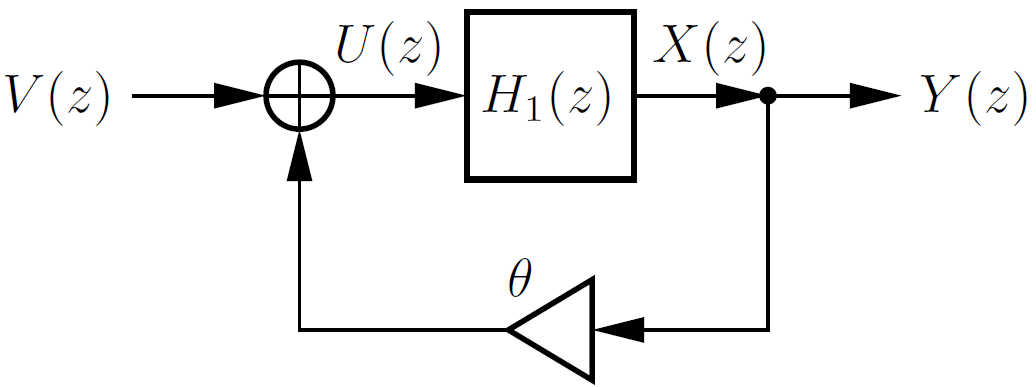
\includegraphics[width=0.35\textwidth]{images_ssp/Outputfeedback}\\
		%	\vspace{0.5 cm}
	\end{minipage}

Gelte $H_1(z) = \frac{\text{Zähler}}{\text{Nenner}}$. Ausgangsrückführung mit dem Skalar $\theta$ liefert nun: $H(z)=\frac{\text{Zähler}}{\text{Nenner} - \text{Zähler}\cdot\theta}$.\\
$\theta$ kann man nun so wählen, sodass das System stabil ist.\\
Einfache Methode zur Stabilisierung eines Systems, jedoch ist nicht jedes System mit skalarer bzw. kausaler Rückkopplung stabilisierbar (z.B. $H(z) = \frac{1}{z^2-3z}$)

\subsection*{Zustandsrückführung}
	\begin{minipage}[t]{0.5\textwidth}
	\hspace{1 cm}
	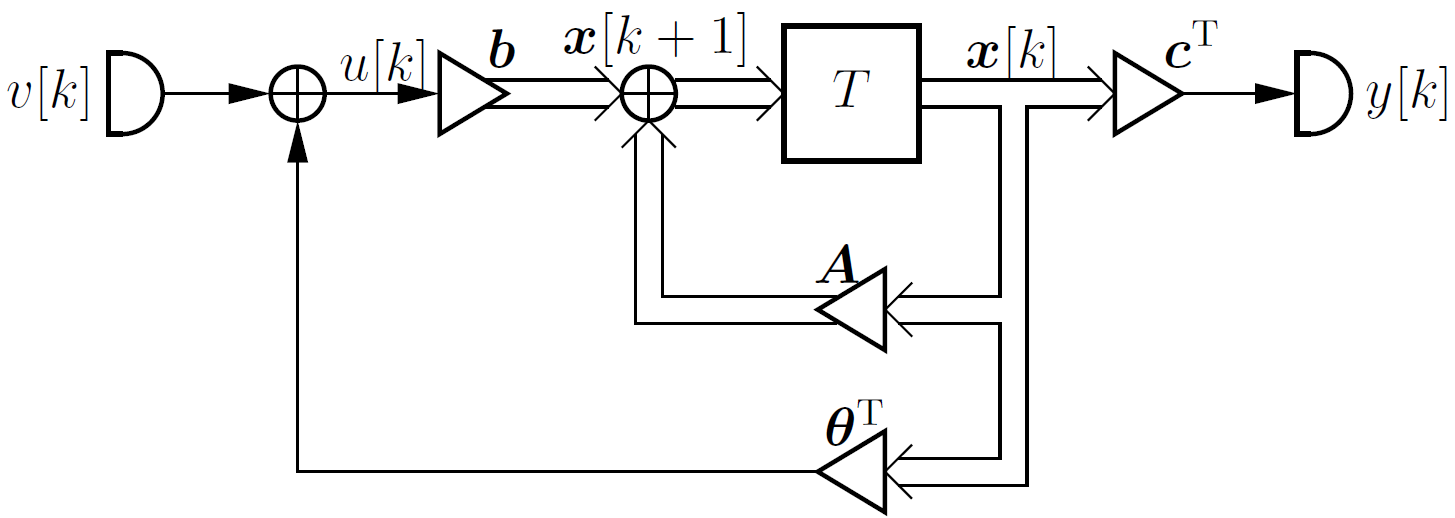
\includegraphics[width=0.45\textwidth]{images_ssp/Statefeedback}\\
	%	\vspace{0.5 cm}
\end{minipage}
Der Durchgriff $d$ beeinflusst die Stabilität nicht, somit betrachten wir Systeme mit $d=0$.\\
Idee: Durch Rückführung der Zustände $\vec x[k]$ mit Gewichtung $\vec \theta$ soll das charakteristische Polynom der Zustandsmatrix so verändert werden, dass alle Eigenwerte stabil sind. Dafür müssen alle Zustände messbar sein.\\

Ist-Polynom (ohne Rückführung):\\
$\alpha(z) = \det(z\ma I - \ma A) = z^n + \alpha_1 z^{n-1} + \dots + \alpha_n$\\
Koeffizientenvektor $\vec \alpha ^T = [\alpha_1,\dots,\alpha_n]^T$\\

Soll-Polynom (mit Rückführung):\\
$\gamma(z) = z^n + \gamma_1 z^{n-1} + \dots + \gamma_n \overset{!}{=}  \det(z\ma I - \ma A - \vec b \vec \theta ^T)$\\
Koeffizientenvektor $\vec \gamma ^T = [\gamma_1,\dots,\gamma_n]^T$\\
Neue Zustandsmatrix des Gesamtsystems: $\ma A' = \ma A + \vec b \vec \theta ^T$\\

$\Rightarrow \boxed{\vec \theta ^T = (\vec \alpha ^T - \vec \gamma ^T) \ma{\mathcal{T}}(\vec \alpha)^{-1} \ma{\mathcal{C}}(\vec b, \ma A)^{-1}}$\\

mit $\ma{\mathcal{T}}(\vec \alpha) = \mat{1 & \alpha_1 & \alpha_2 & \dots & \alpha_{n-1} \\ 0 & 1 & \alpha_1 & \ddots & \\ & \ddots & \ddots & \ddots & \\ 0 & \dots & 0 & 1 & \alpha_1 \\ 0 & \dots & \dots  & 0 & 1}$\\

Somit muss hierfür das System vollst. Steuerbar sein!
\newpage
\subsubsection*{Steuerernormalform}
Ist die Zustandsraumdarstellung wie folgt gegeben:\\
$\ma A = \mat{-\alpha_1 & -\alpha_2 & \dots &-\alpha_{n-1} &-\alpha_n \\ 1 & 0 & \dots & 0 & 0 \\ 0 & 1 & \dots & 0 & 0 \\ \vdots & \vdots & \ddots & \vdots & \vdots \\ 0 & 0 & \dots & 1 & 0}$, 
$\vec b = \mat{1\\0\\0\\ \vdots \\ 0}$\\ 
$\vec c^T = \mat{\beta_1&\beta_2&\beta_3& \dots & \beta_n}^T$\\

$\Rightarrow\vec \theta ^T = (\vec \alpha ^T - \vec \gamma ^T)$\\
\subsubsection*{Diagonalform}
Ist die Zustandsraumdarstellung in Normalform gegeben (wie nach EVD):
$\ma A \rightarrow \ma \Lambda$,\tab $\vec b \rightarrow \vec \mu$,\tab $\vec c^T \rightarrow \vec \eta^T$\\
Ist-Polynom: $\alpha(z) = \prod_{i=1}^n (z-\lambda_i)$, mit $\lambda_i$: Ist-EW\\
Soll-Polynom: $\gamma(z) = \prod_{i=1}^n (z-\kappa_i)$, mit $\kappa_i$: Soll-EW\\

$\Rightarrow\vec \theta_l = -\frac{1}{\mu_l}\frac{\prod_{i=1}^n(\lambda_l - \kappa_i)}{\prod_{i=1, i\ne l}^n(\lambda_l - \lambda_i)}$\\

Dieses Ergebnis ist interessant, wenn man nur einzelne Eigenwerte ändern will. Beispiel:\\
$\kappa_n \ne \lambda_n$, aber für $i<n$: $\kappa_i = \lambda_i$.\\
$\Rightarrow \theta_n = -\frac{1}{\mu_n}(\lambda_n - \kappa_n)$, für $i<n$: $\theta_i = 0$.

\subsection*{Steuerbarkeit zum Ursprung}
Ziel: Bei bekanntem $\vec x[0]$ soll die Eingangsfolge $v[0]$,$v[1]$,$\dots$,$v[n-1]$ so gewählt werden, dass $\vec x[k] = 0$ für $k\ge n$. Dafür muss $v[k]$ wie folgt gewählt werden:\\

$v[k] = -\vec e_n^T\ma{\mathcal{C}}(\vec b, \ma A)^{-1} \ma A^n \vec x[k]$\\
mit $\vec e_n^T = [0,\dots,0,1] \in \mathbb{R}^{1 \times n}$.\\

Dies kann man als eine Zustandsrückführung $v[k] = \vec \theta^T \vec x[k]$ interpretieren, mit $\vec \theta^T = -\vec e_n^T\ma{\mathcal{C}}(\vec b, \ma A)^{-1} \ma A^n$.\\

Diese Wahl von $\theta$ entspricht dem Sollpolynom $\gamma(z) = z^n$, somit werden alle $\lambda_i = 0$ und das System zu einem FIR-Filter.

\subsection*{Asymptotischer Beobachter}
Da man meist nicht alle Zustände messen kann, muss man über die Beobachtung von Eingangs-und Ausgangsfolgen auf die Zustände schließen, um vorherige Methoden anwenden zu können.\\
Angenommen, man kennt die Zustandsraumdarstellung des Systems. Parallel dazu baut ein System mit denselben Parametern $\ma A$, $\vec b$ und $\vec c$, welches eine Schätzfolge $\hat{\vec{x}}[k]$ generiert, die gegen $\vec x[k]$ konvergiert.\\

Die Fehlerfolge $\tilde{\vec{x}}[k] = \vec x[k] - \hat{\vec{x}}[k] = \ma A^k \tilde{\vec{x}}[0]$ konvergiert jedoch nicht gegen Null, wenn das System bereits instabile EW besitzt. Dieses Problem kann man mit Rückführung des Ausgangsfehlers beseitigen:

\begin{minipage}[t]{0.5\textwidth}
	%\vspace{0.1 cm}
	\includegraphics[width=0.55\textwidth]{images_ssp/Asybeo}\\
	%	\vspace{0.5 cm}
\end{minipage}

Nun gilt für die Fehlerfolge:\\
$\tilde{\vec{x}}[k+1] = (\ma A + \vec\varphi \vec c^T)\tilde{\vec{x}}[k]$
Hier kann man ebenfalls ein Sollpolynom $\gamma(z)$ für den Beobachter aufstellen:\\

$\Rightarrow \boxed{\vec \varphi  = \ma{\mathcal{O}}(\vec c^T, \ma A)^{-1}\ma{\mathcal{T}}(\vec \alpha)^{T,-1} (\vec \alpha - \vec \gamma) }$\\

Dies entspricht dem dualen Problem des Reglerdesigns einer Zustandsrückführung.\\
Es gilt: $\ma{\mathcal{O}}(\vec c^T, \ma A) = \ma{\mathcal{C}}(\vec c, \ma A^T)$.
\subsection*{Zustandsraum-Kompensator}
%Dynamischer Zustandsraum-Kompensator
Kombiniert man Zustandsregler und Asymptotischen Beobachter, erhält man den Zustandsraumkompensator:
\begin{minipage}[t]{0.5\textwidth}
	%\vspace{0.1 cm}
	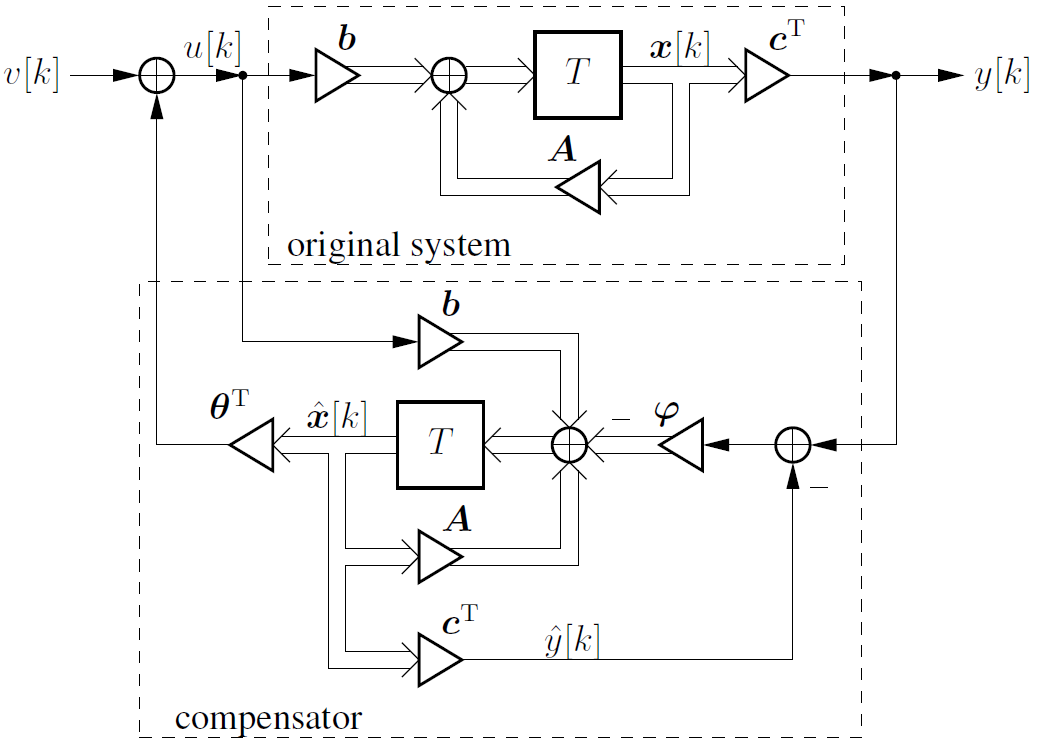
\includegraphics[width=0.55\textwidth]{images_ssp/Compensator}\\
	%	\vspace{0.5 cm}
\end{minipage}
Es gilt:\\
$u[k] = v[k] + \vec \theta ^T \hat{\vec{x}}[k]$, $y[k] = \vec c^T \vec x[k]$, $\hat{y}[k] = \vec c^T \hat{\vec{x}}[k]$\\

$\vec x[k+1] = \ma A \vec x[k] + \vec b \vec \theta^T \hat{\vec{x}}[k] + \vec b v[k]$, mit $\vec x[0] = \vec x_0$\\

$\hat{\vec{x}}[k+1] = -\vec\varphi \vec c^T\vec x[k] + (\ma A + \vec b \vec \theta^T + \vec\varphi \vec c^T) \hat{\vec{x}}[k] + \vec b v[k]$, mit $\hat{\vec{x}}[k] = \hat{\vec{x}}_0$\\

$\tilde{\vec{x}}[k+1] = \vec x[k+1] - \hat{\vec{x}}[k+1] = (\ma A + \vec\varphi \vec c^T)\tilde{\vec{x}}[k]$, mit $\tilde{\vec{x}}[0] = \vec x_0 - \hat{\vec{x}}_0$\\

$\Rightarrow \boxed{ \tilde{\vec{x}}[k] = (\ma A + \vec\varphi \vec c^T)^k \tilde{\vec{x}}[0]}$\\

Zudem gilt:\\
$\boxed{H(z) = \frac{Y(z)}{V(z)} = \vec c^T(z\ma I - \ma A - \vec b \vec \theta ^T)^{-1} \vec b}$\\

Da $H(z)$ nicht von $\vec \varphi$ abhängt und der Schätzfehler $\tilde{\vec{x}}[k]$ nicht von $\vec \theta$ abhängt, können Regler und Beobachter unabhängig voneinander designed werden.\\

Das charakteristische Polynom des Gesamtsystems lautet:
$\alpha_{\text{Gesamt}}(z) = \det(z\ma I - \ma A - \vec \varphi \vec c ^T) \det(z\ma I - \ma A - \vec b \vec \theta ^T)$\\
Das Gesamtsystem ist somit intern stabil, wenn Regler und Beobachter intern stabil sind.
\newpage
%--------------------------------------------------------------------------------------------------------------------------
\section{Statistische Signalverarbeitung}
\subsection*{Suffiziente Statistik}
$\vec X \in \mathbb{C}^m$: Zufallsbeobachtung mit PDF $\text{f}_{\vec X}(\vec x; \vec \theta)$, abhängig vom Parametervektor $\vec \theta \in \mathbb{C}^n$.\\
$\vec T = \vec g(\vec X) \in \mathbb{C}^k$: Statistik.\\

$\rightarrow \vec T$ ist suffizient für $\vec \theta$, wenn gilt:\\
$\boxed{\text{f}_{\vec X|\vec T}(\vec x, \vec t) \neq f(\theta) \Longleftrightarrow \text{f}_{\vec X}(\vec x; \vec \theta) = a(\vec x)b(\vec g(\vec x),\vec \theta)}$\\

Alle Informationen über $\vec \theta$ sind in $\vec T$ enthalten. Somit reicht es, die Statistik $\vec t = \vec g (\vec x)$ anstatt die Messung $\vec x$ zu speichern, falls wir uns nur für $\vec \theta$ interessieren.\\

\ul{Beispiel:} $X_i \sim \mathcal{N}_{\mathbb{C}}(0,\sigma_X^2)$, $\vec X = [X_1,\dots,X_N] \in \mathbb{C}^N$\\
$\rightarrow \text{f}_{\vec X}(\vec x; \sigma_X^2) = \prod\limits_{i=1}^N \text{f}_{X_i}(x_i; \sigma_X^2) =\frac{1}{\pi^N\sigma_X^{2N}} \text{exp}\left(-\sum\limits_{i=1}^{N} \frac{|x_i|^2}{\sigma_X^2}\right)$\\
Mit $t= \sum_{i=1}^{N}|x_i|^2 = ||\vec x||_2^2$:  $b(t,\sigma_X^2 ) = \text{exp}(-\frac{t}{\sigma_X^2})$, $a=1$\\
$\Rightarrow T = ||\vec X||_2^2$ ist eine suffiziente Statistik für $\sigma_X^2$.
\subsection*{Lineares Gauß-Modell}
Für das lineare Gauß-Modell ergibt sich die Zufallsbeobachtung $\vec X$ wie folgt: $\boxed{\vec X = \ma H \vec \theta + \vec N}$\\ mit $\ma H \in \mathbb{C}^{m \times n}$ und $\vec N \sim \mathcal{N}_{\mathbb{C}}(\vec 0, \ma C_{\vec N})$.

\begin{minipage}[h]{0.3\textwidth}
	\hspace{1 cm}
	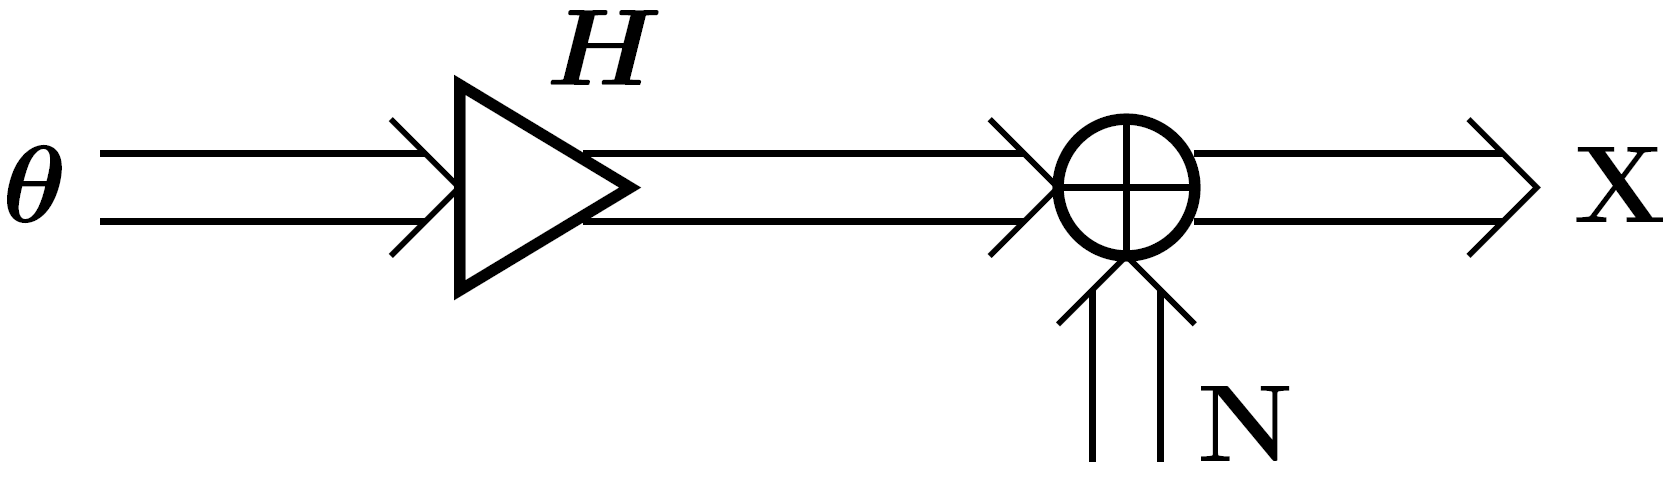
\includegraphics[width=0.55\textwidth]{images_ssp/LinGauMod}\\
\end{minipage}

$\text{f}_{\vec X}(\vec x; \vec \theta) = \frac{1}{\pi^m \det(\ma C_{\vec X})} \text{exp}(-(\vec x - \ma H \vec \theta)^H \ma C_{\vec N}^{-1} (\vec x - \ma H \vec \theta))\\
= \frac{1}{\pi^m \det(\ma C_{\vec X})} \text{exp}(-\vec x ^H \ma C_{\vec N}^{-1} \vec x) \text{exp}(\vec x^H \ma C_{\vec N}^{-1}\ma H \vec \theta \\ \tab \tab \tab + \vec \theta^H \ma H ^H \ma C_{\vec N}^{-1} \vec x - \vec \theta^H \ma H^H \ma C_{\vec N}^{-1} \ma H \vec \theta)$\\

$\Rightarrow \vec T = \ma H^H \ma C_{\vec N}^{-1} \vec X$ ist suffiziente Statistik für $\vec \theta$,\\
mit $\boxed{\ma G_{MF} = \ma H^H \ma C_{\vec N}^{-1}}$ (matched filter).\\

\ul{Hinweis:} Jedes Filter der Form $\ma G_{\text{suffizient}} = \ma A^{-1} \ma G_{MF}$ angewandt auf $\vec X$ liefert eine suffiziente Statistik (mit $\ma A$: beliebige invertierbare Matrix).\\
Somit gilt: $\vec T =  \ma H^H \ma C_{\vec N}^{-1} \ma H \vec \theta + \vec N'$, \\ mit $\vec N' = \ma G_{MF} \vec N \sim \mathcal{N}_{\mathbb{C}}(\vec 0, \ma H^H \ma C_{\vec N}^{-1} \ma H)$. 
\subsubsection*{Linearer Gauß-FIR-Kanal}
\begin{minipage}[h]{0.3\textwidth}
	\hspace{1 cm}
	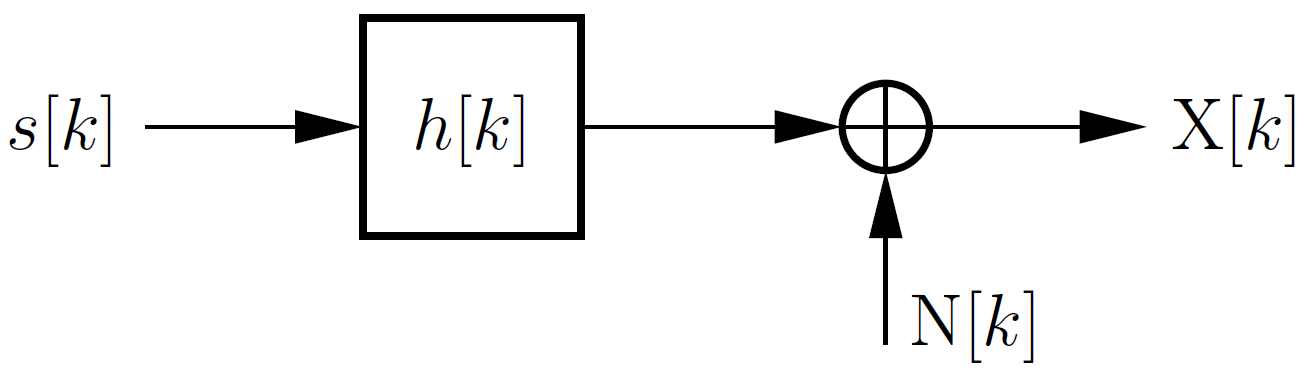
\includegraphics[width=0.55\textwidth]{images_ssp/GauFIR}\\
\end{minipage}
Es gilt $h[k] = \sum_{i=0}^K h_i \delta[k-i]$:\\
$\Rightarrow X[k] = (h*s)[k] + N[k] = \sum_{i=0}^K h_i s[k-i] + N[k]$, wobei das Gaußsche Rauschen $N[k]$ mittelwertfrei und stationär ($E[N[k]N^*[k+\kappa]]$ hängt nur von $\kappa$ ab) sei.\\

Mit $\vec h = [h_0,h_1,\dots,h_K]^T \in \mathbb{C}^{K+1}$:\\
$X[k] = \vec h ^T [s[k], s[k-1], \dots , s[k-K]]^T + N[K]$.\\

Nach $L+1$ aufgenommenen Ausgangswerten $\vec X[k] = [X[k], \dots , X[k-L]]^T \in \mathbb{C}^{L+1}$ ($L \ge K$) erhält man:\\

$\tab \tab \vec X[k] = \ma H \vec s[k] + \vec N[k]$\\

$\ma H = \mat{h_0 & h_1 & h_2 & \dots & h_K & 0 & \dots & 0 \\
0 & h_0 & h_1 & h_2 & \dots & h_K & \dots & 0\\
 & & \ddots & & & & \ddots & {}\\
0 & \dots& 0 &h_0 & & \dots & & h_K}$\\
(Faltungsmatrix $\ma H \in \mathbb{C}^{(L+1) \times (K+L+1)}$)\\
$\vec s[k] = [s[k], \dots, s[k-K-L]]^T \in \mathbb{C}^{K+L+1}$\\
$\vec N[k] = [N[k],\dots, N[k-L]]^T \in \mathbb{C}^{L+1} \sim \mathcal{N}_{\mathbb{C}}(\vec0, \ma C_{\vec N})$\\
\tab \tab mit $\ma C_{\vec N} = E[\vec N[k] \vec N^H[k]]$ unabh. von $k$.\\

\ul{Ziel:} Schätzen der Sequenz $s[k]$. Da $s[k]$ unendlich lang ist, schätzt man in jedem Zeitschritt ein Element aus $s[k]$\\

$\tab \tab \Rightarrow \theta = s[k-d] = \vec e_{d+1}^T \vec s[k]$ \\
mit $d$: Verzögerung, und $\vec e_{d+1} = [0,\dots,1]^T \in \mathbb{R}^{d+1}$.\\

$\text{f}_{\vec X[k]}(\vec x; \vec \theta) = \text{f}_{\vec N[k]}(\vec x - \ma H \vec s[k]) \\
=\frac{1}{\pi^{L+1} \det(\ma C_{\vec N})} \text{exp}(-(\vec x - \ma H \vec s[k])^H \ma C_{\vec N}^{-1} (\vec x - \ma H \vec s[k]))$\\

$\Rightarrow T[k] = \vec e_{d+1}^T \ma H^H \ma C_{\vec N}^{-1} \vec X[k]$ ist suffiz. Statistik für $\theta$.\\

Mit $\vec g^T = [g_0,\dots, g_L] = \vec e_{d+1}^T \ma H^H \ma C_{\vec N}^{-1}$:\\
$T[k] = \vec g^T \vec X[k] = \sum_{l=0}^L g_l X[k-l] = (g*X)[k]$\\
$\Rightarrow$ FIR-Filter: $g[k] = \sum_{l=0}^L g_l \delta[k-l]$\\

\begin{minipage}[h]{0.35\textwidth}
	\hspace{1 cm}
	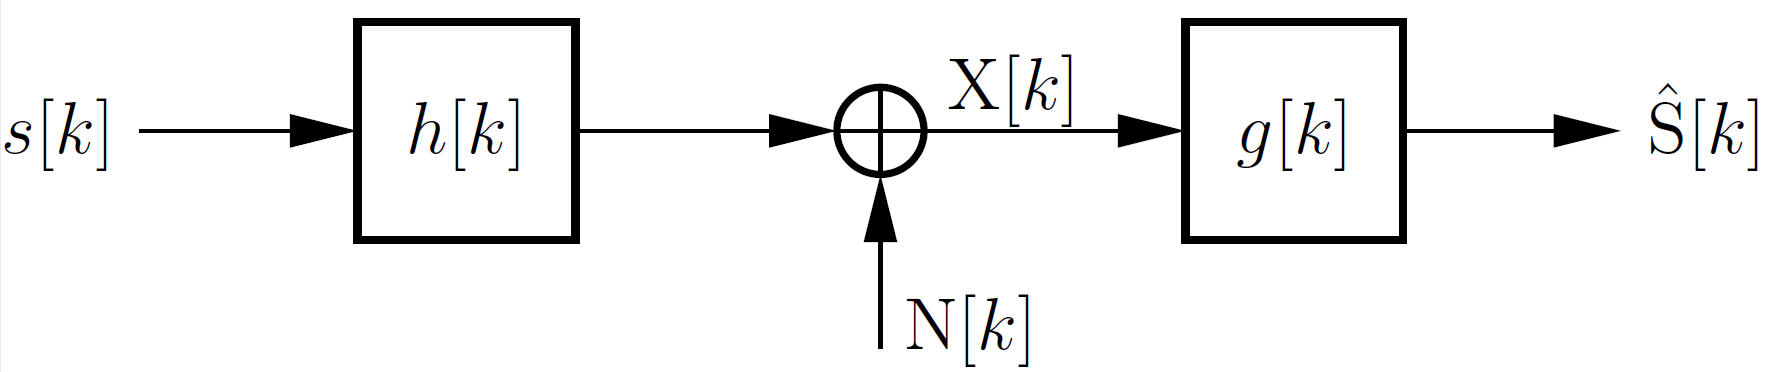
\includegraphics[width=0.55\textwidth]{images_ssp/GauFIR_2}\\
\end{minipage}
Gilt $K \le d \le L$, so enthält die $d+1$-Spalte von $\ma H$ alle Koeffizienten von $h[k] \rightarrow \vec g^T_{MF} = \vec e_{d+1}^T \ma H^H \ma C_{\vec N}^{-1}$\\

Für $\ma C_{\vec N} = \sigma_N^2 \ma I$: $\vec g^T_{MF} = \vec e_{d+1}^T \ma H^H \frac{1}{\sigma_N^2}$. Falls $K=L=d$:\\
$\vec g^T_{MF} =\frac{1}{\sigma_N^2} [h_K^*, \dots, h_0^*] \Longrightarrow g_{MF}[k] = \frac{1}{\sigma_N^2} h^*[d-k]$.
\subsection*{Maximum-Likelihood Schätzung (ML)}
$\hat{\vec x}$: gegebene Realisierung  von $\vec X$.\\
\ul{Idee:} Die PDF wird für gegebenes $\hat{\vec x}$ bezüglich $\vec \theta$ maximiert (PDF als "Wahrscheinlichkeitsmaß" $\rightarrow$ likelihood):\\
$\tab \tab \boxed{\hat{\vec \theta}_{ML} = \underset{\vec \theta}{\text{argmax}} \left( \text{f}_{\vec X}(\hat{\vec x}; \vec \theta) \right)}$\\

Äquivalent zu $\text{f}_{\vec X}$ verwendet man hier oft:\\
-\ul{Likelihood-Funktion:} $l(\vec \theta;\hat{\vec x}) := \text{f}_{\vec X}(\hat{\vec x}; \vec \theta)$\\ (da $\vec \theta$ als Variable betrachtet wird und $\hat{\vec x}$ als Parameter)\\
-\ul{Log-likelihood-Funktion:} $L(\vec \theta;\hat{\vec x}) := \ln l(\vec \theta;\hat{\vec x})$
\subsection*{Maximum A-Posteriori Schätzung (MAP)}
Angenommen, $\vec \theta$ ist auch zufällig $\rightarrow \Theta$ mit PDF $\text{f}_{\vec \Theta}(\vec \theta)$.\\
Für die MAP-Schätzung wird die Verbund-PDF $\text{f}_{\vec X,\vec \Theta}(\vec x, \vec \theta)$ maximiert:\\
$\tab \tab \boxed{\hat{\vec \theta}_{MAP} = \underset{\vec \theta}{\text{argmax}} \left( \text{f}_{\vec X,\vec \Theta}(\hat{\vec x}, \vec \theta) \right)}$\\

Der Satz von Bayes liefert 2 weitere Interpretationen:\\

$\hat{\vec \theta}_{MAP} = \underset{\vec \theta}{\text{argmax }} \text{f}_{\vec X|\vec \Theta}(\hat{\vec x} | \vec \theta) \text{f}_{\vec \Theta}(\vec \theta) = \underset{\vec \theta}{\text{argmax }}\text{f}_{\vec X}(\hat{\vec x}; \vec \theta) \text{f}_{\vec \Theta}(\vec \theta) $\\

$\hat{\vec \theta}_{MAP} = \underset{\vec \theta}{\text{argmax }}  \text{f}_{\vec \Theta|\vec X}(\vec \theta|\hat{\vec x}) \text{f}_{\vec X}(\hat{\vec x}) = \underset{\vec \theta}{\text{argmax }} \text{f}_{\vec \Theta|\vec X}(\vec \theta|\hat{\vec x})$
\newpage

\subsubsection*{ML beim linearen Gauß-Modell}
Die Log-likelihood-Funktion ergibt sich zu:\\
$L(\vec \theta; \vec x) = -(\vec x - \ma H \vec \theta)^H \ma C_{\vec N}^{-1} (\vec x - \ma H \vec \theta) + c$, mit $c$=konst.

$\rightarrow \hat{\vec \theta}_{ML} = \underset{\vec \theta}{\text{argmin}} (\vec x - \ma H \vec \theta)^H \ma C_{\vec N}^{-1} (\vec x - \ma H \vec \theta)$.\\
$\frac{\partial}{\partial \vec \theta^*}(\vec x - \ma H \vec \theta)^H \ma C_{\vec N}^{-1} (\vec x - \ma H \vec \theta) = -\ma H^H\ma C_{\vec N}^{-1} (\vec x - \ma H \vec \theta)\overset{!}{=} 0$\\

$\Rightarrow \hat{\vec \theta}_{ML} = (\ma H^H\ma C_{\vec N}^{-1} \ma H)^{-1}\ma H^H \ma C_{\vec N}^{-1} \vec x$\\

Betrachtet man der Erwartungswert der Schätzung:\\
$E[\vec \Theta_{ML}] = E[(\ma H^H\ma C_{\vec N}^{-1} \ma H)^{-1}\ma H^H \ma C_{\vec N}^{-1} \vec X]\\
= E[(\ma H^H\ma C_{\vec N}^{-1} \ma H)^{-1}\ma H^H \ma C_{\vec N}^{-1} \ma H \vec \theta] \\ + E[(\ma H^H\ma C_{\vec N}^{-1} \ma H)^{-1}\ma H^H \ma C_{\vec N}^{-1} \vec N] = E[\vec \theta] + \vec 0 = \vec \theta$\\
$\tab \Rightarrow $ ML ist erwartungstreu (unbiased)\\
Somit ergibt sich $\hat{\vec \Theta}_{ML} = \vec \Theta + \vec N_{ML}$\\
$\rightarrow \vec N_{ML} = (\ma H^H\ma C_{\vec N}^{-1} \ma H)^{-1}\ma H^H \ma C_{\vec N}^{-1} \vec N$\\ 
$\rightarrow  C_{\vec N_{ML}} = (\ma H^H\ma C_{\vec N}^{-1} \ma H)^{-1}$
\subsubsection*{MAP beim linearen Gauß-Modell}
Die PDF von $\vec \Theta$ muss wie folgt lauten:\\
$\text{f}_{\vec \Theta}(\vec \theta) = \frac{1}{\pi^n \det(\ma C_{\vec \Theta})} \text{exp}(-\vec \theta^H \ma C_{\vec \Theta}^{-1} \vec \theta)$\\
Es gilt $\text{f}_{\vec X,\vec \Theta}(\hat{\vec x}, \vec \theta) = \text{f}_{\vec X|\vec \Theta}(\hat{\vec x} | \vec \theta) \text{f}_{\vec \Theta}(\vec \theta) = \text{f}_{\vec X}(\hat{\vec x}; \vec \theta) \text{f}_{\vec \Theta}(\vec \theta) $\\

$\Rightarrow L(\vec \theta; \vec x) = -(\vec x - \ma H \vec \theta)^H \ma C_{\vec N}^{-1} (\vec x - \ma H \vec \theta) -\vec \theta^H \ma C_{\vec \Theta}^{-1} \vec \theta + \gamma$

$\Rightarrow \hat{\vec \theta}_{MAP} = (\ma H^H\ma C_{\vec N}^{-1} \ma H + \ma C_{\vec \Theta}^{-1})^{-1}\ma H^H \ma C_{\vec N}^{-1} \vec x$\\

Somit gilt nun $\hat{\vec \Theta}_{MAP} \neq \vec \Theta + \vec N_{MAP}$
\subsection*{Least-Squares-Schätzung}
Für lineares Gauß-Modell $\vec X = \ma H \vec \theta + \vec N$:\\
$\tab \boxed{\hat{\vec \theta}_{LS} = \underset{\vec \theta}{\text{argmin }} ||\vec x - \ma H \vec \theta||_2^2}$\\
	
$\rightarrow \frac{\partial}{\partial \vec \theta^*}||\vec x - \ma H \vec \theta||_2^2 = -\ma H ^H \vec x + \ma H ^H \ma H \vec \theta \overset{!}{=} 0$\\

 $\Rightarrow \hat{\vec \theta}_{LS} = (\ma H^H \ma H)^{-1} \ma H^H \vec x = \ma H^+ \vec x$ (Pseudoinv. von $\ma H$)\\
 
LS-Schätzung ist erwartungstreu: $E[\hat{\vec \Theta}_{LS}] = \vec \theta$\\
Für $\ma C_{\vec N} = \sigma_N^2 \ma I$: \tab $\hat{\vec \theta}_{ML} = \hat{\vec \theta}_{LS}$\\
Zudem gilt $\hat{\vec \Theta}_{LS} = \vec \Theta + \vec N_{LS}$\\
$\rightarrow \ma C_{\vec N_{LS}} = (\ma H^H \ma H)^{-1} \ma H^H C_{\vec N} \ma H (\ma H^H \ma H)^{-1}$\\
$\rightarrow \ma C_{\vec N_{LS}} \succeq \ma C_{\vec N_{ML}}$ (Rauschen bei LS größer als bei ML)
\subsection*{Lineare Schätzung}
\ul{Annahme:} Systemmodell und Schätzer sind linear; $\ma C_{\vec N} = E[\vec N \vec N^H]$  bekannt, $E[\vec N] = 0$.\\
($\vec N$ muss nicht gaußverteilt sein!)\\

Der lineare Schätzer $\ma G \in \mathbb{C}^{n \times m}$ liefert:\\
$\tab \tab \boxed{\hat{\vec \Theta} = \ma G \ma X = \ma G \vec \theta + \ma G \vec N}$
\subsubsection*{Best Linear Unbiased Estimator (BLUE)}
\ul{Ziel:} $E[\hat{\vec \Theta}] = \ma G E[\vec X] \overset{!}{=} \vec \theta \Longleftrightarrow \ma G \ma H \vec \theta = \vec \theta$\\
$\tab \Rightarrow \ma G \ma H = \ma I$ \tab (Zero-Forcing-Bedingung)\\

Der BLUE minimiert die Varianz des Schätzers mit der Bedingung der Erwartungstreue:\\
$\ma G_{\text{BLUE}} = \underset{\ma G}{\text{argmin }} \text{var}[\hat{\vec \Theta}] $ u.d.N.: $E[\hat{\vec \Theta}] = \vec \theta $\\
$\Leftrightarrow \ma G_{\text{BLUE}} = \underset{\ma G}{\text{argmin }} \text{spur}(\ma G \ma C_{\vec N} \ma G^H)$ u.d.N.: $\ma G \ma H = \ma I$\\
\tab $\Rightarrow \boxed{ \ma G_{\text{BLUE}} = (\ma H^H\ma C_{\vec N}^{-1} \ma H)^{-1}\ma H^H \ma C_{\vec N}^{-1} }$\\

$\rightarrow$ BLUE = (ML-Schätzung für lin. Gauß-Modell)
\subsubsection*{Minimum Mean Square Error Estimator (MMSE)}
\ul{Ziel:} Mittlerer quadr. Fehler (MSE) wird minimiert.\\
$\vec \Theta$ ist zufällig, $\ma C_{\vec \Theta} = E[\vec \Theta \vec \Theta ^H]$ ist bekannt, $E[\vec \Theta] = 0$, $E[\vec \Theta \vec N ^H] = E[\vec N \vec \Theta ^H] = 0$ ($\rightarrow \vec \Theta$ unabhängig von $\vec N$).\\

Mit $\vec E = \vec \Theta - \hat{\vec \Theta}$ (Fehler): $\boxed{\text{MSE} = \text{var}[\vec E] = E[||\vec \Theta - \hat{\vec \Theta}||_2^2]}$\\
Mit $||\vec y||_2^2 = \vec y^H \vec y = \text{spur}(\vec y \vec y^H)$ und $\hat{\vec \Theta} = \ma G \vec \theta + \ma G \vec N$:\\

$\text{MSE} = \text{spur}(E[(\vec \Theta - \ma G \ma H \vec \Theta - \ma G \vec N)(\vec \Theta - \ma G \ma H \vec \Theta - \ma G \vec N)^H])$\\
$\Rightarrow \boxed{ \text{MSE} = \text{spur}(\ma M (\ma G))}$ \tab  ($\ma M (\ma G)$: MSE-Matrix)\\

Mit $\vec \Theta$ unabhängig von $\vec N$ folgt:\\ $\ma M (\ma G) = (\ma I - \ma G \ma H )\ma C_{\vec \Theta}(\ma I - \ma G \ma H )^H + \ma G \ma C_{\vec N} \ma G ^H$\\
$\rightarrow \ma G_{\text{MMSE}} = \underset{\ma G}{\text{argmin }} \text{MSE}$\\

$ \Rightarrow \boxed{\ma G_{\text{MMSE}} = (\ma H^H\ma C_{\vec N}^{-1} \ma H + \ma C_{\vec \Theta}^{-1})^{-1}\ma H^H \ma C_{\vec N}^{-1}}$\\

(alternativ: $\ma G_{\text{MMSE}} = \ma C_{\vec \Theta} \ma H^H (\ma H\ma C_{\vec \Theta}\ma H^H + \ma C_{\vec N})^{-1}$)\\
$\rightarrow$ MMSE = (MAP-Schätzung für lin. Gauß-Modell)\\

Für $\ma C_{\vec \Theta} = \sigma_{\vec \Theta}^2 \ma I$:\\
$\ma G_{\text{MMSE}} = \sigma_{\vec \Theta}^2 (\ma I +\sigma_{\vec \Theta}^2 \ma H^H\ma C_{\vec N}^{-1} \ma H)^{-1}\ma G_{MF}$ \\
$\Rightarrow \lim\limits_{\sigma_{\vec \Theta}^2 \rightarrow 0} \ma G_{\text{MMSE}} = \vec 0$, \tab $\lim\limits_{\sigma_{\vec \Theta}^2 \rightarrow \infty} \ma G_{\text{MMSE}} = \ma G_{\text{BLUE}}$\\

Für die MSE-Matrix $\ma M(\ma G)$:\\
$\ma M(\ma G) \succeq \ma M_{\text{MMSE}} = \ma M(G_\text{MMSE})$ \\

Der MMSE minimiert somit den $\text{MSE} = \text{spur}(\ma M (\ma G))$ und die resultierende MMSE-Matrix $\ma M_{\text{MMSE}}$ ist das Minimum im Sinne der Definitheit.
\subsection*{MIMO-Detektion}
\begin{minipage}[h]{0.35\textwidth}
	\hspace{1.2 cm}
	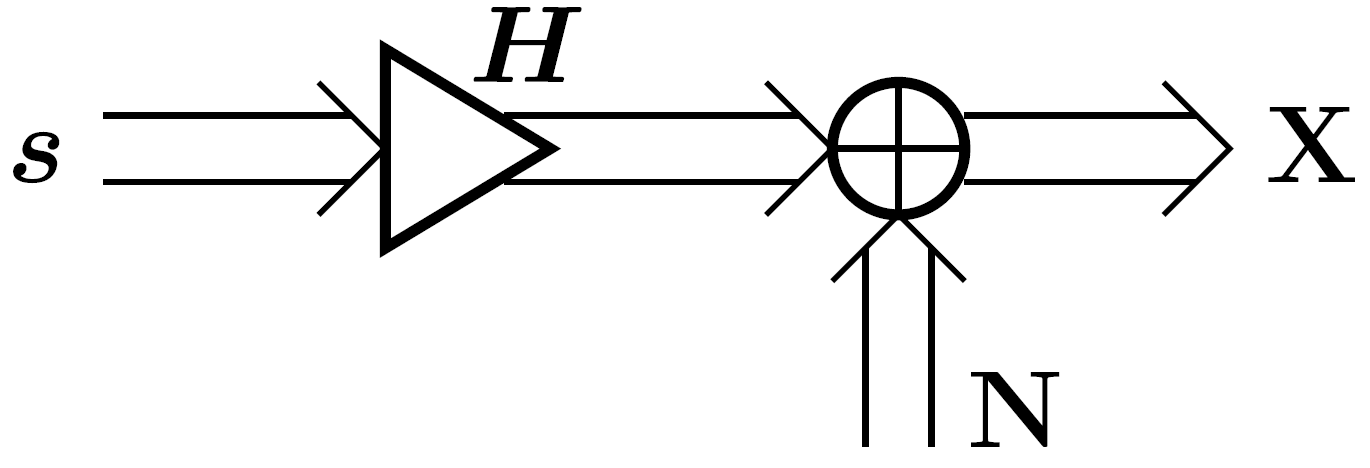
\includegraphics[width=0.55\textwidth]{images_ssp/Mimo}\\
\end{minipage}
$\vec s \in \mathbb{A}^n$: Datensignal (diskrete Werte, z.B. $\mathbb{A}_{\text{BPSK}}=\{-1,1\}$, $\mathbb{A}_{\text{QPSK}}=\{e^{j\frac{\pi}{4}},e^{j\frac{3\pi}{4}},e^{j\frac{5\pi}{4}},e^{j\frac{7\pi}{4}}\}$)\\
$\ma H \in \mathbb{C}^{m\times n}$: MIMO-Kanal ; $\vec N \sim \mathcal{N}_{\mathbb{C}}(\vec 0, \ma C_{\vec N})$.\\
$\Rightarrow \vec X = \ma H \vec s + \vec N \in \mathbb{C}^m$ mit PDF:\\
$\text{f}_{\vec X}(\vec x; \vec s) = \frac{1}{\pi^m \det(\ma C_{\vec N})} \text{exp}(-(\vec x - \ma H \vec s)^H \ma C_{\vec N}^{-1} (\vec x - \ma H \vec s))$
\subsubsection*{ML-Detektion}
$\tilde{\vec s}_{ML} = \underset{\vec s \in \mathbb{A}^n}{\text{argmax}} \left( \text{f}_{\vec X}(\hat{\vec x}; \vec s) \right) = \underset{\vec s \in \mathbb{A}^n}{\text{argmax}} \left( L(\vec s; \vec x) \right)$\\
$\Rightarrow \boxed{\tilde{\vec s}_{ML} = \underset{\vec s \in \mathbb{A}^n}{\text{argmin}} \left( (\vec x - \ma H \vec s)^H \ma C_{\vec N}^{-1} (\vec x - \ma H \vec s) \right)}$
\subsubsection*{Suboptimalität der Symbol-by-Symbol Detektion}
Differenzieren unmöglich, weil $\mathbb{A}$ diskret. Für die Annahme, dass $\mathbb{A} = \mathbb{C}$: Lösen des obigen ML-Problems mittels Wirtinger-Ableitung:\\
$\dfrac{\partial}{\partial \vec s^*}\left( (\vec x - \ma H \vec s)^H \ma C_{\vec N}^{-1} (\vec x - \ma H \vec s) \right) \overset{!}{=} \vec 0$\\
$\Rightarrow \hat{\vec s}_{\text{BLUE}} = (\ma H ^H \ma C_{\vec N}^{-1} \ma H)^{-1} \ma H ^H \ma C_{\vec N}^{-1} \vec x \in \mathbb{C}^n$\\
$\rightarrow$ suffiziente Statistik $\hat{\vec S}_{\text{BLUE}} \sim \mathcal{N}_{\mathbb{C}}(\vec s, (\ma H ^H \ma C_{\vec N}^{-1} \ma H)^{-1})$:\\ 
$\hat{\vec S}_{\text{BLUE}} = \vec s + (\ma H ^H \ma C_{\vec N}^{-1} \ma H)^{-1} \ma H ^H \ma C_{\vec N}^{-1} \vec N $\\
$\Rightarrow \tilde{\vec s}_{ML} = \underset{\vec s \in \mathbb{A}^n}{\text{argmin}} \left( (\hat{\vec s}_{\text{BLUE}} - \vec s)^H \ma H^H \ma C_{\vec N}^{-1}\ma H (\hat{\vec s}_{\text{BLUE}} - \vec s) \right)$\\
Für den Fall, dass $\ma H^H \ma C_{\vec N}^{-1}\ma H$ diagonal:\\
$\tilde{\vec s}_{ML} = \underset{\vec s \in \mathbb{A}^n}{\text{argmin}} \left( \sum\limits_{i=1}^n \alpha_i|\hat s_{\text{BLUE,i}} - s_i|^2 \right) \\ = Q(\hat{\vec s}_{\text{BLUE}}) = [Q(\hat s_{\text{BLUE,1}}), \dots ,Q(\hat s_{\text{BLUE,n}})]^T \in \mathbb{A}^n$\\
mit Quantisierer $Q(x)=\underset{a \in \mathbb{A}}{\text{argmin}} |x-a|^2$, welcher $x$ zum nächsten Element in $\mathbb{A}$ rundet.\\
Das Runden von $\hat{\vec s}_{\text{BLUE}}$ ist nur ML-optimal, wenn $\ma H^H \ma C_{\vec N}^{-1}\ma H$ diagonal ist. Da dies meist nicht diagonal ist, ist die lineare Schätzung gefolgt von dem Symbol-by-Symbol Quantisierer allgemein suboptimal.\\ $\rightarrow$ lineare Schätzung ist suboptimal.
\subsubsection*{MMSE-Metrik}
ML-Detektor minimiert die ML-Metrik:\\
$\mu_{ML}(\vec s) = (\hat{\vec s}_{\text{BLUE}} - \vec s)^H \ma H^H \ma C_{\vec N}^{-1}\ma H (\hat{\vec s}_{\text{BLUE}} - \vec s)$\\
Die MMSE-Metrik lautet:\\
$\mu_{MMSE}(\vec s) = (\hat{\vec s}_{\text{MMSE}} - \vec s)^H (\ma I + H^H \ma C_{\vec N}^{-1}\ma H )(\hat{\vec s}_{\text{MMSE}} - \vec s)$\\
wobei $\hat{\vec S}_{\text{MMSE}} = (\ma I + H^H \ma C_{\vec N}^{-1}\ma H ) H^H \ma C_{\vec N}^{-1} \vec X$.\\
$\Rightarrow \tilde{\vec s}_{\text{MMSE}} =  \underset{\vec s \in \mathbb{A}^n}{\text{argmin}} \left( \mu_{MMSE}(\vec s) \right) $\\
$\rightarrow \tilde{\vec s}_{\text{MMSE}} = \tilde{\vec s}_{\text{ML}}$ wenn $\mathbb{A}$ Konstant-Modulus Alphabet
\subsubsection*{Sphere Decoder}
ML- und MMSE-Metrik allgemein:\\
$\mu(\vec s) = (\hat{\vec s} - \vec s)^H \ma A (\hat{\vec s} - \vec s)$, mit $\ma A \in \mathbb{C}^{n\times n}$\\
$\ma A$ ist nicht-negativ definit $\rightarrow$ Cholesky-Zerlegung: \\$\ma A = \ma L^H \ma D \ma L$ mit $\ma L \in \mathbb{C}^{n\times n}$: untere Dreiecksmatrix (1er auf Diagonale) und $\ma D \in \mathbb{R}_{+,0}^{n\times n}$: nicht-negative Diagonalmatrix.\\
$\Rightarrow \mu(\vec s) = ||\ma D^{1/2}(\ma L \hat{\vec s} - \ma L \vec s)||_2^2 =  ||\ma D^{1/2}(\hat{\vec x} - \ma L \vec s)||_2^2$\\
Wegen der Dreiecksstruktur von $\ma L$ folgt: ($\hat x_i = \vec e_i^T \ma L \hat{\vec s}$)\\
$\Rightarrow \mu(\vec s) = \sum\limits_{i=1}^n d_{i,i} \big | \hat x_i - s_i - \sum\limits_{j=1}^{i-1} l_{i,j}s_j \big | ^2$\\
$\rightarrow \mu_1(\vec s) = d_{1,1} |\hat s_1 - s_1|^2$\\
$\rightarrow \mu_2(\vec s) = d_{2,2} |\hat s_2 - s_2 + l_{2,1}(\hat s_1 - s_1)|^2$ usw..\\
$\mu_i$ hängt nur von $s_1, \dots, s_i$ ab, somit kann man die Minimierung von $\mu(s)$ als eine Suche nach dem Pfad mit minimaler totaler Metrik $\sum_{i=1}^{n} \mu_i(\vec s)$ interpretieren:\\
\begin{minipage}[h]{0.6\textwidth}
	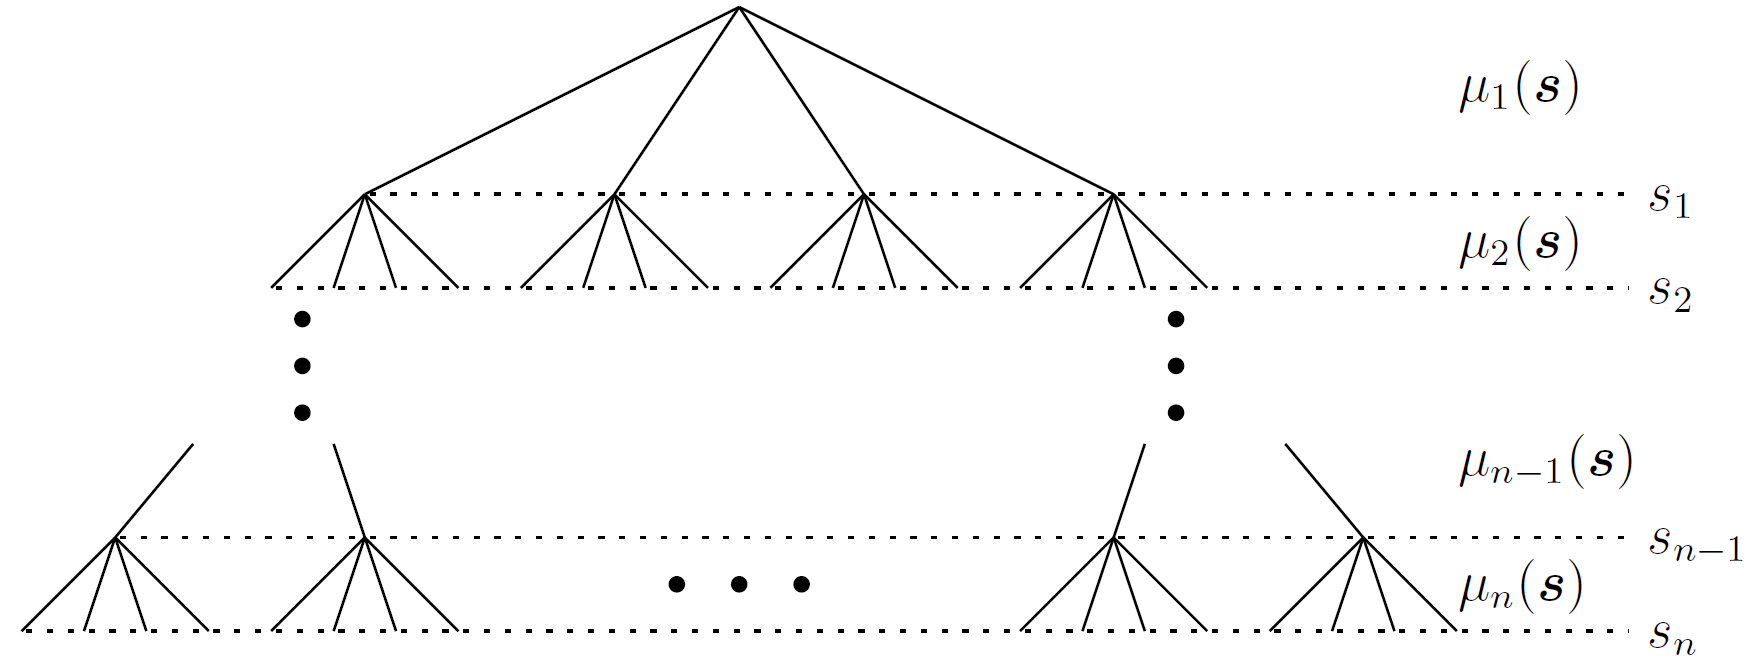
\includegraphics[width=0.55\textwidth]{images_ssp/Baum}\\
\end{minipage}
%--------------------------------------------------------------------------------------------------------------------------
\section{Anhang}
\begin{cookbox}{Optimierung mit Nebenbedingungen}
	\begin{itemize}
		\item[1)] Problem muss folgende Form haben:\\
		$\vec x_{\text{opt}} = \underset{\vec x}{\text{argmin }}f(\vec x) $ u.d.N.: $\vec g(\vec x) = \vec 0$\\
		mit $\vec x \in \mathbb{C}^n$, $f(\vec x) \in \mathbb{R}$, $\vec g (\vec x) \in \mathbb{C}^m$, $m\le n$
		\item[2)] Lagrangefunktion aufstellen:\\ $L(\vec x, \vec \lambda) = f(\vec x) + 2 \text{Re }\{\vec \lambda^H \vec g(\vec x)\}\\ = f(\vec x) + \vec \lambda^H \vec g(\vec x) + \vec g(\vec x)^H\vec \lambda$, mit $\vec \lambda \in \mathbb{C}^m$
		\item[3)] $\dfrac{\partial}{\partial \vec x^*} L(\vec x, \vec \lambda) = 0$ berechnen und nach $\vec x(\vec \lambda)$ umformen
		\item[4)] $\vec x(\vec \lambda)$ in Nebenbedingung  $\vec g(\vec x) = \vec 0$ einsetzen und nach $\vec \lambda$ umformen
		\item[5)] $\vec \lambda$ in $\vec x(\vec \lambda)$ einsetzen $\Rightarrow \vec x_{\text{opt}}$
	\end{itemize}
\end{cookbox}
-----------------------------------------------------------------------\\
\ma{\underline{Quelle:}} Skriptum zur Vorlesung Systeme der Signalverarbeitung von Dr. M. Joham, Professur MSV, TUM.
\newpage
%--------------------------------------------------------------------------------------------------------------------------
\end{multicols}
\end{document}









